%% LyX 2.5.1 created this file.  For more info, see https://www.lyx.org/.
%% Do not edit unless you really know what you are doing.
\documentclass[journal,article,submit,moreauthors]{Definitions/mdpi}
\usepackage{textcomp}
\usepackage[utf8]{inputenc}
\usepackage{colortbl}
\usepackage{float}
\usepackage{url}
\usepackage{varwidth}
\usepackage{amsmath}
\usepackage{graphicx}

\makeatletter

%%%%%%%%%%%%%%%%%%%%%%%%%%%%%% LyX specific LaTeX commands.

\Title{Parallel Optimized Particle Swarm Optimization: An Efficient Parallel
Approach for Neural Network Training}

\Author{Konstantinos G. Barkas$^{*}$, Ioannis G. Tsoulos$,$ Vasileios Charilogis,
and Glykeria Kyrou}


\address{Department of Informatics and Telecommunications, University of Ioannina,
47150 Kostaki Artas, Greece\\
}


\corres{Author to whom correspondence should be addressed.}


\abstract{Global optimization has become a cornerstone of modern machine learning,
particularly for the challenging task of training high-dimensional
neural network architectures. Despite the prevalence of established
metaheuristics, traditional approaches frequently struggle with the
irregular and multimodal error surfaces inherent in complex training
landscapes. This paper proposes the Parallel Optimized Particle Swarm
Optimization (OPSO), a multi-population parallel framework specifically
engineered to enhance the training efficiency and predictive accuracy
of neural networks across classification and regression tasks. OPSO
integrates several advanced mechanisms: a simulated annealing-based
acceptance criterion to escape local minima, adaptive inertia weights
that dynamically respond to stagnation by injecting momentum, and
a hybrid Broyden--Fletcher--Goldfarb--Shanno (BFGS) local search
phase for fine-grained convergence. By partitioning the swarm into
interacting sub-populations and leveraging modern multi-core architectures,
OPSO significantly reduces training time while achieving superior
generalization compared to classical PSO and state-of-the-art methods.
Experimental evaluations demonstrate that OPSO consistently converges
to more robust solutions, outperforming baseline models on demanding
and irregular error surfaces. These results underscore OPSO as a highly
efficient and scalable framework for optimizing neural network parameters
in complex search spaces.}


\keyword{Parallel Metaheuristics; Particle Swarm Optimization (OPSO); Neural
Network Training; Global Optimization; Hybrid Local Search; Adaptive
Inertia; Simulated Annealing}

\DeclareTextSymbolDefault{\textquotedbl}{T1}
%% Because html converters don't know tabularnewline
\providecommand{\tabularnewline}{\\}
%% Variable width box for table cells
\newenvironment{cellvarwidth}[1][t]
    {\begin{varwidth}[#1]{\linewidth}}
    {\@finalstrut\@arstrutbox\end{varwidth}}

%%%%%%%%%%%%%%%%%%%%%%%%%%%%%% User specified LaTeX commands.
%  LaTeX support: latex@mdpi.com 
%  For support, please attach all files needed for compiling as well as the log file, and specify your operating system, LaTeX version, and LaTeX editor.

%=================================================================
%\documentclass[preprints,article,submit,moreauthors]{Definitions/mdpi} 
% For posting an early version of this manuscript as a preprint, you may use "preprints" as the journal. Changing "submit" to "accept" before posting will remove line numbers.

% Below journals will use APA reference format:
% admsci, aieduc, behavsci, businesses, econometrics, economies, education, ejihpe, famsci, games, humans, ijcs, ijfs, investment, fclam, jintelligence, journalmedia, jrfm, jsam, languages, opermanag, peacestud, pmh, psycholint, publications, tourismhosp, youth

% Below journals will use Chicago reference format:
% arts, genealogy, histories, humanities, laws, literature, religions, risks, socsci

%--------------------
% Class Options:
%--------------------
%----------
% journal
%----------
% Choose between the following MDPI journals:
% accountaudit, acn, acoustics, actuators, addictions, addictprev, adhesives, adolescents, aerobiology, aerospace, agriculture, agriengineering, agrochemicals, agronomy, ai, aichem, aieng, aimater, aimed, aipa, air, aisens, aisoc, algorithms, allergies, alloys, amh, analog, analytica, analytics, anatomia, anesthres, animals, antibiotics, antibodies, antioxidants, applbiosci, appliedchem, appliedmath, appliedphys, applmech, applmicrobiol, applnano, applsci, aps, aquacj, archaeolstud, architecture, arm, arthropoda, asc, asi, astronautics, astronomy, atmosphere, atoms, audiolres, automation, axioms, bacteria, batteries, bdcc, beverages, biochem, bioengineering, biologics, biology, biomass, biomechanics, biomed, biomedicines, biomedinformatics, biomimetics, biomolecules, biophysica, bioresourbioprod, biosensors, biosphere, biotech, birds, blockchains, bloods, blsf, brainsci, breath, buildings, cancers, carbon, cardio, cardiogenetics, cardiovascmed, catalysts, cells, ceramics, challenges, chemengineering, chemistry, chemosensors, chemproc, children, chips, cimb, civileng, cleantechnol, climate, clinbioenerg, clinpract, clockssleep, cmd, cmtr, coasts, coatings, colloids, colorants, commodities, complexities, complications, compounds, computation, computers, condensedmatter, conservation, constrmater, cosmetics, covid, crops, cryo, cryptography, crystals, csmf, ctn, culture, curroncol, cyber, dairy, data, ddc, dentistry, dermato, dermatopathology, designs, devices, dhi, diabetology, diagnostics, dietetics, digital, disabilities, diseases, diversity, dna, drones, drugreact, drylands, dynamics, earth, ebj, ecm, ecologies, edm, eesp, electricity, electrochem, electronicmat, electronics, embodiedintell, encyclopedia, endocrines, energies, eng, engproc, entomology, entropy, environments, environremediat, epidemiologia, epigenomes, esa, est, fermentation, fibers, fintech, fire, fishes, fluids, foodeng, foods, forecasting, forensicsci, forests, fossstud, foundations, fractalfract, freshwater, fuels, future, futureinternet, futurepharmacol, futurephys, futuretransp, galaxies, gases, gastroent, gastrointestdisord, gastronomy, gels, genes, geochem, geographies, geohazards, geomatics, geometry, geosciences, geotechnics, geriatrics, germs, glacies, grainsci, grasses, green, greenhealth, gucdd, gynecolcancer, hardware, hazardousmatters, healthcare, healthcmater, hearts, hemato, hematolrep, hep, heritage, higheredu, highthroughput, horticulturae, hospitals, hydrobiology, hydrogen, hydrology, hydrometeorology, hydropower, hygiene, idr, iic, ijem, ijerph, ijgi, ijmd, ijms, ijns, ijom, ijp, ijpb, ijt, ijtm, ijtpp, ijtst, ime, immuno, industries, inflammj, informatics, information, infrastructures, inorganics, insects, instruments, inventions, iot, j, jaestheticmed, jal, japma, jcdd, jcm, jcp, jcrm, jcs, jcto, jdad, jdb, jdream, jemr, jeta, jfb, jfmk, jfth, jgbg, jgg, jimaging, jlpea, jmahp, jmmp, jmms, jmp, jmse, jne, jnt, jof, joi, joitmc, joma, jop, joptm, jor, jox, jpbi, jphytomed, jpm, jsan, jtaer, jvd, jzbg, kidneydial, kinasesphosphatases, knowledge, labmed, laboratories, lam, land, lasers, legumes, life, lights, limnolrev, lipidology, liquids, livers, logics, logistics, lubricants, lymphatics, machines, macromol, magnetism, magnetochemistry, make, marinedrugs, maritime, materials, materproc, mathematics, mca, mcb, measurements, medicina, medicines, medsci, membranes, merits, metabolites, metals, meteorology, methane, metrics, metrology, micro, microarrays, microbiolres, microelectronics, micromachines, microorganisms, microplastics, microwave, minerals, mining, mmphys, modelling, molbank, molecules, mollusca, mps, msf, mti, multimedia, muscles, nanoenergyadv, nanomanufacturing, nanomaterials, ncrna, ndt, network, neuroglia, neuroimaging, neurolint, neurosci, nitrogen, notspecified, nursrep, nutraceuticals, nutrients, obesities, occuphealth, oceans, ohbm, onco, optics, oral, organics, organoids, osteology, oxygen, pandemics, parasites, parasitologia, particles, pathogens, pathophysiology, pediatrrep, pets, pharmaceuticals, pharmaceutics, pharmacoepidemiology, pharmacy, phc, philosophies, photochem, photonics, photovoltaics, phycology, physchem, physics, physiologia, plants, plasma, platforms, pollutants, polymers, polysaccharides, populations, poultry, powders, precision, precisoncol, preprints, proceedings, processes, prosthesis, proteomes, psf, psychiatryint, psychoactives, purification, quantumrep, quaternary, qubs, radiation, rareearths, rdt, reactions, realestate, receptors, recycling, regeneration, remotesensing, reports, reprodmed, resources, rheumato, rjpm, robotics, rsee, ruminants, safety, sanpp, sca, sci, scipharm, sclerosis, seeds, sensors, separations, sexes, shi, signals, sinusitis, siuj, skins, smartcities, smartfish, sna, societies, software, soilsystems, solar, solids, spectroscj, sports, standards, stats, std, stratsediment, stresses, strokerep, superintelligence, surfaces, surgeries, suschem, sustainability, sustainfoods, sustainpackag, symmetry, synbio, systems, tae, targets, taxonomy, technologies, telecom, test, textiles, thalassrep, therapeutics, thermo, timespace, tomography, toxics, toxins, tph, transplantology, transportation, traumacare, traumas, tri, tropicalmed, universe, urbansci, uro, vaccines, vehicles, venereology, vetsci, vibration, virtualworlds, viruses, vision, waste, water, welding, wem, wevj, wild, wind, women, world, zoonoticdis

%---------
% article
%---------
% The default type of manuscript is "article", but can be replaced by: 
% abstract, addendum, article, book, bookreview, briefreport, casereport, comment, commentary, communication, conferenceproceedings, correction, conferencereport, entry, expressionofconcern, extendedabstract, datadescriptor, editorial, essay, erratum, hypothesis, interestingimage, obituary, opinion, projectreport, reply, retraction, review, perspective, protocol, shortnote, studyprotocol, systematicreview, supfile, technicalnote, viewpoint, guidelines, registeredreport, tutorial
% supfile = supplementary materials

%----------
% submit
%----------
% The class option "submit" will be changed to "accept" by the Editorial Office when the paper is accepted. This will only make changes to the frontpage (e.g., the logo of the journal will get visible), the headings, and the copyright information. Also, line numbering will be removed. Journal info and pagination for accepted papers will also be assigned by the Editorial Office.

%------------------
% moreauthors
%------------------
% If there is only one author the class option oneauthor should be used. Otherwise use the class option moreauthors.

%=================================================================
% MDPI internal commands - do not modify
\firstpage{1} 
\setcounter{page}{\@firstpage}
\pubvolume{1}
\issuenum{1}
\articlenumber{0}
\pubyear{2026}
\copyrightyear{2026}
%\externaleditor{Firstname Lastname} % More than 1 editor, please add `` and '' before the last editor name
\datereceived{}
\daterevised{ } % Comment out if no revised date
\dateaccepted{}
\datepublished{}
%\datecorrected{} % For corrected papers include a "Corrected: XXX" date in the original paper.
%\dateretracted{} % For retracted papers include a "RETRACTED: XXX" date in the original paper.
%\doinum{} % Used for some special journals, like molbank
%\pdfoutput=1 % Uncommented for upload to arXiv.org
%\CorrStatement{yes}  % For updates
%\longauthorlist{yes} % For many authors that exceed the left citation part
%\IsAssociation{yes} % For association journals

%=================================================================
% Add packages and commands here. The following packages are loaded in our class file: fontenc, inputenc, calc, indentfirst, fancyhdr, graphicx, epstopdf, lastpage, ifthen, lineno, float, amsmath, setspace, enumitem, mathpazo, booktabs, titlesec, etoolbox, tabto, xcolor, soul, multirow, microtype, tikz, totcount, changepage, attrib, upgreek, cleveref, amsthm, hyphenat, natbib, hyperref, footmisc, url, geometry, newfloat, caption

%=================================================================
%% Please use the following mathematics environments: Theorem, Lemma, Corollary, Proposition, Characterization, Property, Problem, Example, ExamplesandDefinitions, Hypothesis, Remark, Definition, Notation, Assumption
%% For proofs, please use the proof environment (the amsthm package is loaded by the MDPI class).

%=================================================================
% The fields PACS, MSC, and JEL may be left empty or commented out if not applicable
%\PACS{J0101}
%\MSC{}
%\JEL{}

%%%%%%%%%%%%%%%%%%%%%%%%%%%%%%%%%%%%%%%%%%
% Only for the journal Diversity
%\LSID{\url{http://}}

%%%%%%%%%%%%%%%%%%%%%%%%%%%%%%%%%%%%%%%%%%
% Only for the journal Applied Sciences:
%\featuredapplication{Authors are encouraged to provide a concise description of the specific application or a potential application of the work. This section is not mandatory.}
%%%%%%%%%%%%%%%%%%%%%%%%%%%%%%%%%%%%%%%%%%

%%%%%%%%%%%%%%%%%%%%%%%%%%%%%%%%%%%%%%%%%%
% Only for the journal Data:
%\dataset{DOI number or link to the deposited data set in cases where the data set is published or set to be published separately. If the data set is submitted and will be published as a supplement to this paper in the journal Data, this field will be filled by the editors of the journal. In this case, please make sure to submit the data set as a supplement when entering your manuscript into our manuscript editorial system.}

%\datasetlicense{license under which the data set is made available (CC0, CC-BY, CC-BY-SA, CC-BY-NC, etc.)}

%%%%%%%%%%%%%%%%%%%%%%%%%%%%%%%%%%%%%%%%%%
% Only for the journal BioTech, Fishes, Neuroimaging and Toxins
%\keycontribution{The breakthroughs or highlights of the manuscript. Authors can write one or two sentences to describe the most important part of the paper.}

%%%%%%%%%%%%%%%%%%%%%%%%%%%%%%%%%%%%%%%%%%
% Only for the journal Encyclopedia
%\encyclopediadef{Instead of the abstract}
%\entrylink{The Link to this entry published on the encyclopedia platform.}
%%%%%%%%%%%%%%%%%%%%%%%%%%%%%%%%%%%%%%%%%%

%%%%%%%%%%%%%%%%%%%%%%%%%%%%%%%%%%%%%%%%%%
% Different journals have different requirements. Please check the specific journal guidelines in the "Instructions for Authors" on the journal's official website.
 
%\addhighlights{yes}
%\renewcommand{\addhighlights}{%
%
%\noindent This is an optional section, the goal of which is to increase the discoverability and readability of the article via search engines and other scholars. Highlights should not be a copy of the abstract, but a simple overview allowing the reader to quickly and simply find out what the article is about and what can be cited from it. Each of these parts should be up to 2 bullet points.\vspace{3pt}\\
%\textbf{What are the main findings?}
% \begin{itemize}[labelsep=2.5mm,topsep=-3pt]
% \item First bullet.
% \item Second bullet.
% \end{itemize}\vspace{3pt}
%\textbf{What are the implications of the main findings?}
% \begin{itemize}[labelsep=2.5mm,topsep=-3pt]
% \item First bullet.
% \item Second bullet.
% \end{itemize}
%}
\usepackage[ruled,vlined,linesnumbered]{algorithm2e}
\usepackage{tikz}
\usetikzlibrary{fit, arrows.meta}
\usepackage[font=small,labelfont=bf]{caption}

\makeatother

\begin{document}
\maketitle

\section{Introduction}

The training of Artificial Neural Networks (ANNs) represents one of
the most critical and challenging tasks in modern machine learning
and computational intelligence \citep{Zhang2023,Kaveh2022}. From
a mathematical perspective, training an ANN is formulated as a large-scale
global optimization problem \citep{Charilogis2024}, where the objective
is to minimize an error function by adjusting the network’s weights
and biases. The global optimization problem is defined as: 

\begin{equation}
\mathbf{x}^{*}=\arg\min_{\mathbf{x}\in S}f(\mathbf{x})
\end{equation}
where the search space $\ensuremath{S}$ is defined as the high-dimensional
hyper-rectangle:

\[
S=[a_{1},b_{1}]\otimes[a_{2},b_{2}]\otimes\cdots\otimes[a_{n},b_{n}]
\]
In the context of neural network training, the objective function
$\ensuremath{\ensuremath{\ensuremath{f(\mathbf{x})}}}$ represents
the loss function (e.g., Mean Squared Error or Cross-Entropy), and
the vector $\ensuremath{\boldsymbol{x}\in\mathbb{R}^{n}}$ contains
the network's parameters. This optimization landscape is highly non-linear,
non-convex, and multi-modal, containing an immense number of local
minima \citep{Dauphin2014}. Apart from neural network training, this
mathematical formulation finds critical applications in a variety
of real-world problems, such as physics \citep{Metropolis1953,Carleo2017},
chemistry \citep{Xia2025}, economics \citep{BuenoFerrer2025}, and
medicine \citep{Andres2025,Shehata2025}. Historically, optimization
methods are divided into two main categories: deterministic and stochastic.
Deterministic approaches, such as Interval methods \citep{Fernandez2022,Gillner2026}
or gradient-based algorithms (e.g., Backpropagation, Stochastic Gradient
Descent, Adam), rely on mathematical proofs or gradient derivatives
to navigate the search space \citep{Goodfellow2016}. However, in
high-dimensional and non-convex neural network landscapes, gradient-based
methods are heavily prone to getting trapped in saddle points or sub-optimal
local minima and are highly sensitive to initial weight configurations
\citep{Dauphin2014,Rumelhart1986,Goodfellow2016}. To overcome these
limitations, stochastic and metaheuristic methods have been widely
adopted. Guided by randomness, these methods do not guarantee finding
the absolute global minimum in polynomial time, but they consistently
locate high-quality solutions with remarkable implementation simplicity
\citep{Yang2020}. \\
Researchers have proposed numerous stochastic algorithms, including
Controlled Random Search \citep{Price1977}, Simulated Annealing \citep{Kirkpatrick1983,Kuo2022},
Differential Evolution \citep{Storn1997}, Particle Swarm Optimization
(PSO) \citep{Gad2022,Poli2007}, Ant Colony Optimization \citep{Dorigo2006},
and Genetic Algorithms \citep{Holland1992}. Furthermore, modern computational
paradigms have successfully ported these algorithms to multi-core
and GPU architectures to accelerate high-dimensional optimization
\citep{Essaid2019,Cano2016}, with comprehensive surveys available
in recent literature \citep{Houssein2024,Sun2022}. \\
Among these metaheuristics, Particle Swarm Optimization (PSO) has
emerged as a highly efficient population-based algorithm inspired
by the social behavior of bird flocking \citep{Salgotra2026}. In
PSO, a population of candidate solutions, called particles, explores
the search space $S$. Each particle $i$ is characterized by its
current position $\boldsymbol{x_{i}}$ and its velocity \textbf{$\boldsymbol{v}_{\boldsymbol{i}}$}.
The dynamic movement of each particle in a $D$-dimensional space
is governed by updating its velocity and position at each iteration
step \citep{Poli2007,Kennedy1995} according to the following formulation:

\begin{equation}
v_{i,d}=\omega\cdot v_{i,d}+c_{1}\cdot r_{1}\cdot(\mathbf{p}_{\text{best},i,d}-x_{i,d})+c_{2}\cdot r_{2}\cdot(\mathbf{g}_{\text{best},d}-x_{i,d})
\end{equation}

\begin{equation}
x_{i,d}=x_{i,d}+v_{i,d}
\end{equation}
where $\ensuremath{\omega}$ is the inertia weight introduced to control
the impact of the previous velocity \citep{Shi1998}, $c_{1}$ and
$c_{2}$ are the cognitive and social acceleration coefficients, and
$\ensuremath{r_{1},r_{2}\sim U(0,1)}$ are uniformly distributed random
numbers. The vector $\ensuremath{\mathbf{p}_{\text{best},i}}$denotes
the personal best position discovered by particle $i$, while $\ensuremath{\ensuremath{\mathbf{g}_{\text{best}}}}$represents
the global best position found by the entire swarm. Despite its success,
classical PSO can suffer from premature convergence and high computational
costs when optimizing complex neural network architectures, falling
into local minima during the exploitation phase \citep{Gad2022,Poli2007}.
Many researchers focus on dynamically adjusting the inertia weight
$\ensuremath{\omega}$ \citep{Rathore2017,Charilogis2022} or integrating
hybrid and parallel implementation techniques \citep{Demelomenezes2022,Charilogis2023}
to tackle complex numerical optimization problems. However, limited
attention has been given to the simultaneous enhancement of scalability,
multi-population parallel evolution, and adaptive convergence control
in large-scale optimization environments. To address these challenges,
this paper introduces the Parallel Optimized Particle Swarm Optimization
(Parallel OPSO) method, specifically engineered to enhance the training
efficiency and predictive accuracy of neural networks. The proposed
algorithm is a multi-population parallel framework that partitions
the swarm into interacting sub-populations, leveraging modern multi-core
architectures to significantly reduce execution time.\\

The novelty of Parallel OPSO lies in the integration of several advanced
mechanisms within a unified parallel framework:
\begin{itemize}
\item Simulated Annealing Acceptance Criterion: A stochastic acceptance
criterion is integrated to allow particles to occasionally accept
worse positions, enabling the swarm to escape stubborn local minima
\citep{Kirkpatrick1983,Kuo2022}.
\item Adaptive Inertia Weight and Momentum: The inertia weight $\ensuremath{\omega}$
dynamically responds to swarm stagnation by injecting momentum, balancing
wide-range exploration and local exploitation based on the algorithm's
real-time performance \citep{Charilogis2022}.
\item Hybrid Local Search Phase: Incorporates a deterministic BFGS quasi-Newton
method to refine promising candidate solutions and significantly enhance
convergence accuracy toward the global optimum \citep{Nocedal2006}.
\end{itemize}
The main contributions of this work are summarized as follows: 
\begin{itemize}
\item A parallel cooperative extension of the PSO algorithm, where the swarm
is partitioned into multiple sub-populations evolving simultaneously
on multi-core architectures using the OpenMP framework to enhance
exploration in large-scale search spaces.
\item A dynamic propagation mechanism that enables structured and controlled
information exchange among the independent subpopulations, improving
convergence speed while maintaining overall population diversity.
\item The incorporation of adaptive inertia weight $\ensuremath{\omega}$
based on the framework introduced in \citep{Charilogis2022}, which
dynamically responds to swarm stagnation by injecting momentum, effectively
balancing global exploration and local exploitation based on the algorithm's
real-time performance.
\item The integration of a Simulated Annealing-based stochastic acceptance
criterion \citep{Kirkpatrick1983,Kuo2022}, which allows particles
to occasionally accept worse positions, providing a robust mechanism
to escape stubborn local minima.
\item The incorporation of a hybrid local search phase utilizing the deterministic
BFGS quasi-Newton method \citep{Nocedal2006} to significantly improve
convergence accuracy and speed up the localization of the exact global
optimum.
\item A comprehensive experimental evaluation spanning both large-scale
global optimization benchmark problems and demanding neural network
training tasks for classification and regression, demonstrating that
Parallel OPSO consistently converges to more robust solutions compared
to state-of-the-art algorithms.
\end{itemize}
The remainder of this article is organized as follows: Section \ref{sec:Materials-and-Methods}
outlines the foundational background of classical PSO alongside the
detailed mathematical formulation of the proposed Parallel OPSO; Section
\ref{sec:Results} presents the experimental setup, benchmark functions,
and comparative performance analysis; and finally, Section \ref{sec:Conclusions}
summarizes our key findings, provides concluding remarks, and outlines
directions for future research.

\section{Materials and Methods\label{sec:Materials-and-Methods}}

This section initiates with the main aspects of the original PSO method
and continues by presenting in detail the main parts of the proposed
method.

\subsection{\textbf{Classical Particle Swarm Optimization (PSO)}}

The classical Particle Swarm Optimization (PSO) algorithm, originally
introduced by Kennedy and Eberhart \citep{Kennedy1995}, is a population-based
stochastic optimization technique inspired by the social behavior
of bird flocking or fish schooling. The algorithm explores an $n$-dimensional
continuous search space $\ensuremath{\mathcal{S}\subset\mathbb{R}^{n}}$
using a population of $m$ interacting agents called particles. Each
particle $i$ ($i\in\{1,2,\ldots,m\})$ is characterized by its dynamic
state parameters, consisting of an $n$-dimensional position vector
$\ensuremath{\mathbf{x}_{i}}=\left[x_{i1},x_{i2},\ldots,x_{in}\right]^{T}$and
a corresponding velocity vector$\ensuremath{\ensuremath{\ensuremath{\mathbf{v}_{i}}=\left[v_{i1},v_{i2},\dots,v_{in}\right]^{T}.}}$During
the optimization process, each particle maintains a memory of its
own historical personal best position discovered so far, denoted as
$\ensuremath{\mathbf{p}_{i}}=\left[p_{i1},p_{i2},\dots,p_{in}\right]^{T}$.
Concurrently, the swarm tracks the absolute global best position achieved
by any particle in the entire population, defined as$\ensuremath{\mathbf{p}_{\text{gbest}}=\arg\min_{i\in\{1,\dots,m\}}f\left(\mathbf{p}_{i}\right)}$,
where$f(\cdot)$ represents the objective function under minimization.
To balance global exploration and localized exploitation, a trade-off
extensively evaluated in recent metaheuristic literature \citep{Kaveh2022,Charilogis2024},
Shi and Eberhart \citep{Shi1998} introduced the inertia weight factor
$\ensuremath{\omega}$. At each discrete evolutionary epoch $\text{\ensuremath{t}}$,
the dynamic trajectories of the particles are updated according to
the following stochastic kinematic equations: 

\begin{equation}
\mathbf{v}_{i}(t+1)=\omega(t)\cdot\mathbf{v}_{i}(t)+c_{1}\cdot\mathbf{r}_{1}\cdot\left(\mathbf{p}_{i}(t)-\mathbf{x}_{i}(t)\right)+c_{2}\cdot\mathbf{r}_{2}\cdot\left(\mathbf{p}_{\text{gbest}}(t)-\mathbf{x}_{i}(t)\right)
\end{equation}

\begin{equation}
\mathbf{x}_{i}(t+1)=\mathbf{x}_{i}(t)+\mathbf{v}_{i}(t+1)
\end{equation}
where $\ensuremath{\omega(t)}$ is the inertia weight, $c_{1}$ and
$c_{2}$ denote the cognitive and social acceleration coefficients,
respectively, and$\ensuremath{\mathbf{r}_{1},\mathbf{r}_{2}\sim\mathcal{U}(0,1)}$
represent independent uniformly distributed random vectors injected
to maintain stochastic diversity. Despite its mathematical simplicity
and high convergence speed, the classical formulation is prone to
stagnation in complex multimodal landscapes due to rapid loss of population
diversity, a challenge frequently highlighted in modern optimization
benchmarks \citep{Rebello2021,Gad2022}. The main parts of the original
PSO method are listed in Algorithm \ref{alg:classical_pso}.\\

\begin{algorithm}[H]
\caption{The classical PSO algorithm.}
\label{alg:classical_pso}
\DontPrintSemicolon

\tcc{Initialization Phase}
\textbf{Set} $\text{iter} \gets 0$ (iteration counter)\;
\textbf{Set} the population size $m$ and maximum iterations allowed $\text{iter}_{\max}$\;
\textbf{Initialize} randomly the positions of the $m$ particles $x_1, x_2, \dots, x_m$, with $x_i \in \mathcal{S} \subset \mathbb{R}^n$\;
\textbf{Initialize} randomly the velocities of the $m$ particles $v_1, v_2, \dots, v_m$\;
\For{$i \gets 1$ \KwTo $m$}{
    $p_i \gets x_i$ \tcp*{Store best personal position}
}
\textbf{Find} $g = \arg\min_{i \in \{1, \dots, m\}} f(x_i)$ and \textbf{set} $p_{\text{gbest}} \gets x_g$\;

\tcc{Main Evolutionary Loop}
\While{$\text{iter} < \text{iter}_{\max}$}{
    \For{$i \gets 1$ \KwTo $m$}{
        \textbf{Update} the velocity $v_i$ via Eq.~(4)\;
        \textbf{Update} the position $x_i$ via Eq.~(5)\;
        \textbf{Evaluate} the fitness of particle $i$, $f(x_i)$\;
        \If{$f(x_i) \le f(p_i)$}{
            $p_i \gets x_i$\;
        }
    }
    \textbf{Find} $g = \arg\min_{i \in \{1, \dots, m\}} f(p_i)$ and \textbf{set} $p_{\text{gbest}} \gets p_g$\;
    $\text{iter} \gets \text{iter} + 1$\;
}
\KwRet{$p_{\text{gbest}}, f(p_{\text{gbest}})$}
\end{algorithm}

\subsection{\textbf{Parallel Optimized Particle Swarm Optimization Algorithm}\protect \\
}

The distributed framework of the Optimized Particle Swarm Optimization
(OPSO) algorithm is engineered by partitioning the global agent population
into $K$ distinct subpopulations and it is presented graphically
in Figure \ref{fig:Parallel-OPSO-framework}. Each subpopulation operates
as an autonomous evolutionary unit allocated to an individual processing
element, enabling simultaneous execution across a shared-memory environment
\citep{OpenMP2024}. 
\begin{figure}[H]
\centering
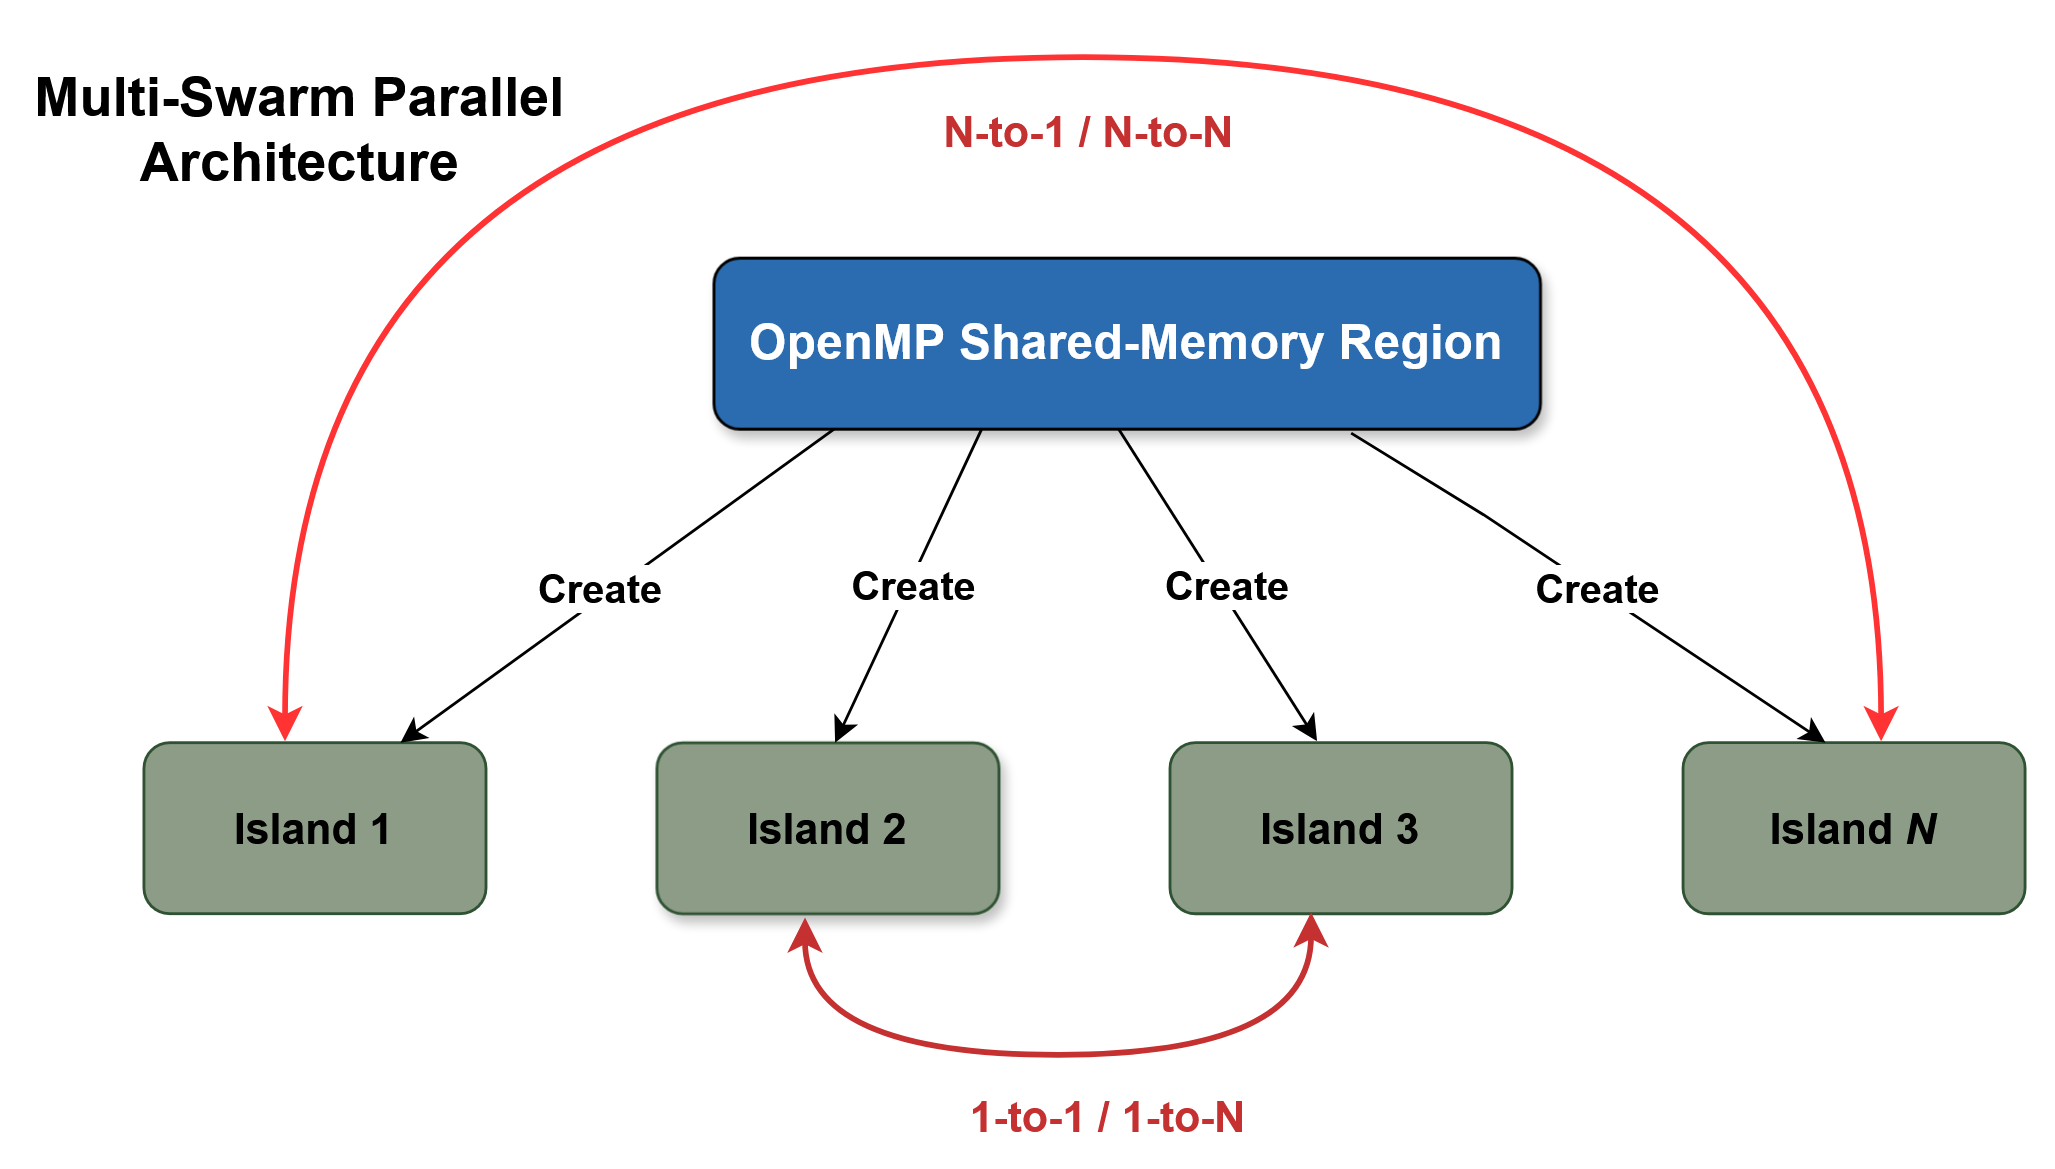
\includegraphics[width=0.85\columnwidth]{parallel_pso_islands}\caption{{\footnotesize Parallel OPSO framework illustrating thread distribution
and flexible inter-island migration topologies.\label{fig:Parallel-OPSO-framework}}}

\end{figure}

 Before initiating the optimization cycle, the multi-swarm configurations
are established, and the global termination strategy $\mathrm{(TS)}$
is selected. To govern decentralized convergence behavior and manage
interaction dynamics between the concurrently evolving swarms, the
architecture introduces a set of control features: a topological propagation
method $(\mathrm{NM)}$, a generational communication rate $(\mathrm{NR)}$,
a volumetric quantity of migrated solutions $(\mathrm{NP)}$, and
a localized termination criterion $(\mathrm{TC)}$ \citep{Charilogis2023,Kyrou2026}.\\

The communication frequency across the multi-swarm layout is controlled
by the propagation rate $(\mathrm{NR)}$, which establishes the exact
number of generational steps between consecutive data distributions.
Low values for $\mathrm{NR}$ enforce tight coupling and frequent
interaction, a configuration that can accelerate convergence velocities
but risks collapsing population diversity \citep{Kyrou2026,daSilveira2020}.
Conversely, high values for $\mathrm{NR}$ grant the individual islands
extended periods of decoupled execution, fostering independent exploration
of unmapped solution regions.\\
\\
In a similar manner, the volume of shared elite information is dictated
by the parameter $\mathrm{NP}$, which defines the number of top-performing
vectors transmitted during a migration step. Expanding $\mathrm{NP}$
strengthens the collective exploitation capability by injecting high-quality
geometric coordinates into target swarms; however, excessive data
injection can induce premature convergence by steering all independent
groups toward identical local optima \citep{Kyrou2026,daSilveira2020,Abadlia2017}.
Within this framework, the specific bounds for $\mathrm{NR}$ and
$\mathrm{NP}$ are derived through systematic empirical tuning to
maintain a healthy balance between localized search refinement and
global space exploration, with the precise values detailed in the
Experimental Results section.\\
\\
During every generational step, the system monitors each subpopulation
to determine if it has met its localized termination criterion $\mathrm{(TC)}$,
which is evaluated independently via an advanced convergence heuristic
known as the Similarity check\citep{Tsoulos2021}. The total number
of stagnated units is then cross-referenced with a macro-level decision
threshold, denoted as $Q$. This threshold mathematically operationalizes
the chosen system-wide termination strategy $\mathrm{(TS)}$ to govern
the macro-level optimization loop\citep{Kyrou2026,Tsoulos2021}:

\begin{equation}
Q=\begin{cases}
1, & \text{if }TS=ANY\\
\lfloor K/2\rfloor+1, & \text{if }TS=MAJORITY\\
K, & \text{if }TS=ALL
\end{cases}
\end{equation}
Following the calculation of the threshold metrics, the subpopulations
proceed with their parallel evolutionary operations, executing localized
kinematics updates and simulated annealing leader adjustments. At
generational intervals matching the propagation rate $(\mathrm{NR)}$,
the system triggers the designated migration topology $(\mathrm{NM})$
to distribute $\mathrm{NP}$ elite candidate vectors across the multi-threaded
network\citep{Charilogis2023,Kyrou2026,Abadlia2017}.\\
\\
The iteration counter increments, and the status of the threshold
criterion $Q$ is evaluated. If the conditions for global termination
are not fulfilled, the concurrent optimization sequence continues.
Upon satisfying the macro-level stopping condition, the framework
invokes a memetic refinement sequence, executing a rigorous local
search directly around the global best solution$\ensuremath{g_{\text{best}}}$to
secure high-precision mathematical accuracy before returning the final
optimized result \citep{Petalas2007}.\\
\\
From an architectural standpoint, mapping each subpopulation to an
isolated thread or processing core facilitates true concurrent execution.
Synchronization barriers are strictly confined to the scheduled propagation
phases, allowing the swarms to evolve independently during intermediate
generations and significantly minimizing memory access latencies \citep{Charilogis2023}.
Resource utilization is optimized through the selection of the global
termination strategies (ANY, MAJORITY, ALL), which prevent thread
starvation and idle processing states by eliminating the requirement
for all processing elements to terminate at the same time. The ANY
strategy, in particular, permits rapid continuation by halting the
global loop the moment early convergence is detected on any single
thread via the Similarity metric \citep{Tsoulos2021}. Furthermore,
the computational footprint of the migration phase remains small,
as it restricts communication to a limited set of elite solution coordinates.
This brief coordination phase introduces negligible latency relative
to the overall objective function evaluation costs, and it significantly
enhances optimization performance by enabling effective information
sharing across the parallel architecture \citep{Charilogis2023,Kyrou2026}.

\subsection{\textbf{Inter-Swarm Communication Protocol and Migration Topologie}s\protect \\
}

Within the cooperative execution phase of the parallel framework,
the communication layer facilitates the distribution of high-quality
parameter configurations among the concurrent islands. When the scheduled
migration interval conditions are satisfied, the elite solution vectors
identified by a specific subpopulation are transmitted across the
shared-memory space to overwrite the lowest-performing coordinates
of the designated target swarms. The foundational objective of this
information routing scheme is to optimize cross-island exploration,
ensuring that promising topological discoveries are rapidly assimilated
into the broader optimization landscape to enhance overall convergence
efficiency \citep{Charilogis2023,Kyrou2026}.\\
Unlike conventional distributed metaheuristics that rely on static
and rigid structural layouts, such as ring, star, or fully-mesh migration
topologies, the proposed framework introduces a localized, dynamically
configurable migration model tailored for high-dimensional execution
spaces. Conventional geometric topologies impose strict synchronization
locks and significant thread contention penalties as the execution
scale grows, which frequently induces severe memory access latencies
within shared-memory architectures \citep{Charilogis2023,Kyrou2026}.
To avoid structural complexity and eliminate excessive communication
overhead, the parallel architecture relies on a versatile routing
protocol operating across four discrete configuration states:
\begin{itemize}
\item One-to-One ($1\text{to}1$): A single source subpopulation, selected
uniformly at random, migrates its historical elite parameter states
exclusively to a single target subpopulation, which is also designated
through a random uniform distribution.
\item One-to-All ($1\text{to}N$): A randomly isolated subpopulation serves
as a central broadcaster, transmitting its optimal geometric updates
to refresh the search vectors of all other $K-1$ active swarms simultaneously.
\item All-to-One ($N\text{to}1$): Every active computational swarm routes
its current top-performing vectors toward a single, randomly targeted
subpopulation, consolidating global directional data into a localized
spatial window to catalyze structural exploitation.
\item All-to-All ($N\text{to}N$): A dense execution mode where every individual
subpopulation synchronizes and exchanges its finest candidate solutions
with the historical memory matrix of every other swarm in the network.\\
\\
By adjusting the combination of these topological routing strategies
$(\mathrm{NM)}$ alongside the volumetric payload parameter $(\mathrm{NP)}$,
the OPSO framework maintains a fluid balance between regional exploitation
and global population diversity \citep{Charilogis2023,Kyrou2026}.
This dynamic coordination mitigates structural stagnation risks while
preserving the low coordination footprint required for efficient execution
on multi-core compute clusters.\\
\end{itemize}

\subsection{\textbf{Adaptive Inertia weight mechanism}}

To achieve a self-regulating balance between global exploration and
localized exploitation, each autonomous subpopulation discards static
or strictly time-dependent parameter scaling. Instead, an Adaptive
Inertia Weight Mechanism is implemented \citep{Rathore2017}, adapting
the phenotypic stagnation-tracking framework introduced in the Ideal
Particle Swarm Optimization (IPSO) architecture \citep{Charilogis2022}.
This framework evaluates the state of the swarm by monitoring the
phenotypic convergence rate across consecutive generations. When the
global fitness gradient flattens, indicating that the multi-swarm
trajectory is confined within a local attractor, the inertia weight
parameter is dynamically adjusted to modulate particle momentum.\\
\\
Operationally, the system calculates the absolute differential progress
of the collective fitness landscape at every iteration. If the fitness
deviation between sequential states falls below a predefined threshold,
a stagnation counter increments. By calculating the ratio of cumulative
stagnant states against the elapsed generational counter, a dynamic
constraint coefficient is derived. Consequently, when the subpopulation
actively discovers novel structural minima, the velocity profile maintains
a high exploratory momentum. Conversely, when severe multi-island
stagnation is detected, the inertia scales down to its minimum operating
boundary, dampening particle velocities to focus computational resources
strictly on high-precision local exploitation\citep{Rathore2017,Charilogis2022}.\\


\subsubsection{\textbf{\textit{Mathematical Formulation}}}

The evolutionary state monitoring is governed by evaluating the global
fitness volume change at each generation $\text{\ensuremath{t}}$,
tracking structural stagnation vectors as formalized in the IPSO framework
\citep{Charilogis2022}:

\begin{equation}
\delta(t)=\left|\sum^{m}_{i=1}f_{i}(t)-\sum^{m}_{i=1}f_{i}(t-1)\right|
\end{equation}
where $\ensuremath{m}$ denotes the number of particles within the
subpopulation, and $\ensuremath{f_{i}(t)}$ represents the objective
cost value of the $\ensuremath{i}$-th particle at generation $t$.
The localized stagnation state indicator $\ensuremath{\zeta(t)}$
is defined as:

\begin{equation}
\zeta(t)=\begin{cases}
1, & \text{if }\delta(t)=0\\
0, & \text{otherwise}
\end{cases}
\end{equation}
Using the real-time feedback from $\ensuremath{\zeta(t)}$, the cumulative
stagnation tracking matrix $\ensuremath{S_{\delta}(t)}$ and its corresponding
density ratio $C_{\delta}(t)$ are computed dynamically:

\begin{equation}
S_{\delta}(t)=\sum^{t}_{k=1}\zeta(k)
\end{equation}

\begin{equation}
C_{\delta}(t)=\frac{S_{\delta}(t)}{t}
\end{equation}
The adaptive inertia weight $\ensuremath{\omega(t)}$ supplied to
the velocity kinematic updating core is formally governed by the bound-constrained
formulation\citep{Charilogis2022}, building upon the dynamic inertia
weight control concepts introduced in \citep{Shi1998}:

\begin{equation}
\omega(t)=\max\left(\omega_{\min},\min\left(\omega_{\max},\omega_{\max}-C_{\delta}(t)\cdot(\omega_{\max}-\omega_{\min})\right)\right)
\end{equation}
where $\omega_{\max}$ and $\omega_{\min}$ represent the predefined
boundary coefficients governing the dynamic momentum spectrum.\\


\subsection{\textbf{Adaptive Simulated Annealing Acceptance Criterion}}

To balance the exploitation of local optima with the necessity of
maintaining exploratory pressure, a stochastic acceptance mechanism
is integrated into the leader update phase of each island. Traditional
PSO variants typically employ a greedy selection rule, which often
leads to rapid convergence toward suboptimal regions in non-convex,
high-dimensional landscapes \citep{Poli2007,Salgotra2026}. To mitigate
this, our approach implements an Adaptive Simulated Annealing Acceptance
Criterion, allowing the sub-population leader ($\boldsymbol{P}_{\text{best},k}$)
to occasionally accept inferior solutions based on a temperature-dependent
probability inspired by the classic Simulated Annealing framework
\citep{Metropolis1953,Kirkpatrick1983,Kuo2022}.\\
Let $\Delta=f(\mathbf{X}_{\text{best},k})-f(\mathbf{P}_{\text{best},k})$
represent the fitness difference between the current best particle
within sub-cluster $S_{k}$ and the recorded sub-cluster leader. The
probability$\ensuremath{P_{\text{acc}}}$of accepting a potentially
worse configuration is defined as:\\
\begin{equation}
P_{\text{acc}}=\begin{cases}
1.0, & \text{if }\Delta<0\\[6pt]
\exp\left(-\frac{\Delta}{T\cdot\bar{\Delta}_{k}+\epsilon}\right), & \text{otherwise}
\end{cases}
\end{equation}
\\
where $T$ represents the current normalized temperature under a linear
cooling schedule, calculated as $T=\max\left(1.0-\text{progress},10^{-4}\right)$
to enforce a minimum thermal floor, with$\ensuremath{\text{progress}}$denoting
the relative execution progress ($t/t_{\max}$). To ensure robustness
across diverse objective function scales, an adaptive scaling factor
$\overline{\Delta}_{k}$ is maintained locally for each sub-cluster
$k$, updating incrementally via an Exponential Moving Average (EMA)
as $\ensuremath{\bar{\Delta}_{k}\leftarrow0.9\cdot\bar{\Delta}_{k}+0.1\cdot\Delta}$
for every positive fitness delta observed. The term $\epsilon=10^{-9}$
serves as a numerical stability constant to prevent division by zero.\\
This mechanism facilitates a transition from a high-exploration phase
at the onset of the optimization process, where the acceptance of
inferior moves enables the algorithm to escape local attractors,to
a high-exploitation phase as $T$ approaches zero, effectively narrowing
the search towards the global optimum \citep{Kirkpatrick1983,Kuo2022}.
By decoupling the leader update from strict greedy selection, the
algorithm exhibits enhanced resilience against the \textquotedbl saddle
point\textquotedbl{} problem in high-dimensional spaces \citep{Dauphin2014},
ensuring a more thorough traversal of the search space before settling
into a terminal configuration \citep{Fernandez2022,Gillner2026}.
This adaptive control, combined with the parallel island-model paradigm,
provides a robust defense against premature stagnation without the
prohibitive computational overhead associated with global, non-localized
simulated annealing schedules \citep{Charilogis2022,Charilogis2023,daSilveira2020,Abadlia2017}.

\subsection{\textbf{Hybrid Local Search Phase}}

To balance global stochastic exploration with high-precision exploitation,
Parallel OPSO incorporates a memetic hybrid local search phase \citep{Petalas2007}
based on the deterministic Broyden--Fletcher--Goldfarb--Shanno
(BFGS) quasi-Newton algorithm \citep{Nocedal2006}. During execution,
the local search procedure is stochastically triggered on the global
best position$\ensuremath{\mathbf{g}_{\text{best}}}$with a predefined
probability $p_{ls}$$\texttt{(\texttt{local\_search\_rate}).}$Additionally,
a final deterministic refinement step is mandatorily executed inside
the $\texttt{done()}$routine upon meeting the swarm stopping criteria.
The BFGS algorithm iteratively refines the target position vector
$\ensuremath{\mathbf{x}_{k}}$ along a search direction $\ensuremath{\mathbf{p}_{k}=-H_{k}\nabla f(\mathbf{x}_{k})}$,
where $H_{k}$ represents an approximate inverse Hessian matrix. At
each local step $k$, $H_{k}$ is dynamically updated using the spatial
difference vector$\ensuremath{\mathbf{s}_{k}}=\ensuremath{\mathbf{x}_{k+1}}-\ensuremath{\mathbf{x}_{k}}$
and the gradient difference vector $\ensuremath{\mathbf{y}_{k}=\nabla f(\mathbf{x}_{k+1})-\nabla f(\mathbf{x}_{k})}$
according to:

\begin{equation}
H_{k+1}=(I-\rho_{k}\mathbf{s}_{k}\mathbf{y}^{T}_{k})H_{k}(I-\rho_{k}\mathbf{y}_{k}\mathbf{s}^{T}_{k})+\rho_{k}\mathbf{s}_{k}\mathbf{s}^{T}_{k}
\end{equation}
 where $\ensuremath{\rho_{k}=(\mathbf{y}^{T}_{k}\mathbf{s}_{k})^{-1}}$.
This gradient-based coupling guarantees superlinear local convergence
characteristics, refining the stochastic candidate solutions of OPSO
to exact numerical optima.

\subsection{\textbf{Subpopulation Termination Criterion via Similarity Check\label{subsec:similarity-check}}}

In parallel multi-swarm architectures, determining the optimal execution
boundary for each autonomous subpopulation is critical. Halting an
island prematurely deprives the global swarm of valuable population
diversity and high-quality coordinates during migration phases \citep{daSilveira2020,Abadlia2017}.
Conversely, allowing a stagnated subpopulation to execute until the
global maximum iteration limit leads to wasted processor cycles and
unnecessary energy consumption \citep{Charilogis2023,Kyrou2026}.
To resolve this trade-off, each individual island $k$ dynamically
monitors its own search trajectory via a localized termination state
$\mathrm{(\text{TC}_{k})}$.\\
\\
To ensure sufficient initial exploration and avoid false-positive
termination signals caused by early stochastic fluctuations, a mandatory
warm-up period is enforced. Localized convergence diagnostics remain
inactive until the generation counter satisfies:

\begin{equation}
t\ge t_{\min},\quad\text{where }t_{\min}=50
\end{equation}
Upon crossing this threshold, the algorithm tracks the fitness progression
of island $k$ at every generation $t$ by calculating the absolute
difference between its current and previous local best objective values:

\begin{equation}
\Delta f_{k}(t)=\left|f(\mathbf{L}_{\text{best},k}(t))-f(\mathbf{L}_{\text{best},k}(t-1))\right|
\end{equation}
To evaluate whether $\ensuremath{\Delta f_{k}(t)}$ reflects genuine
mathematical convergence rather than a transient plateau, the framework
embeds the Similarity Check heuristic proposed by Tsoulos et al. \citep{Tsoulos2021}.
Conventional termination metrics often rely on instantaneous point-to-point
differences, making them highly sensitive to noise in complex fitness
landscapes. In contrast, the Similarity Check evaluates the convergence
behavior over a sliding historical window of $\ensuremath{W=25}$
consecutive iterations. Specifically, island $k$ is declared locally
converged ($TC_{k}=\text{true}$) when the average objective improvement
falls below a predefined tolerance threshold $\varepsilon$:

\begin{equation}
\frac{1}{W}\sum^{W-1}_{m=0}\Delta f_{k}(t-m)<\epsilon
\end{equation}
From an implementation perspective, each parallel worker thread maintains
an isolated heuristic evaluator instance ($\texttt{threadSimilarity[\ensuremath{k}]}$).
This design eliminates thread contention and lock overheads, enabling
fully decoupled convergence checks across processing cores \citep{OpenMP2024,Charilogis2023}.
The aggregate count of stagnated islands is continuously tracked as:

\begin{equation}
S_{\text{term}}=\sum^{K}_{k=1}\mathbb{I}(\text{TC}_{k}=\text{true})
\end{equation}
where $\mathbb{I}(\cdot)$ denotes the indicator function. When $\ensuremath{S_{\text{term}}\ge Q},$the
global termination strategy $\ensuremath{(\text{TS})}$ is triggered
\citep{Kyrou2026,Tsoulos2021}. Finally, the maximum iteration count
$\ensuremath{t_{\max}}$ serves as an absolute safety ceiling ($\ensuremath{t\ge t_{\max}}$),
guaranteeing bounded computational time under all execution conditions.

\subsection{\textbf{Pseudocode and Algorithmic Summary}}

The complete metaheuristic workflow of the proposed Parallel Optimized
Particle Swarm Optimization algorithm, incorporating the parallel
migration topologies, adaptive inertia weight control mechanisms,
simulated annealing leader acceptance criteria, and hybrid local search
refinement, is synthesized in the following pseudocode, presented
across three parts to preserve legibility: the initialization phase
(Algorithm \ref{alg:opso-init}), the main evolutionary loop (Algorithm
\ref{alg:opso-main}), and the per-island parallel update procedure
invoked within it (Algorithm \ref{alg:opso-island}):

\begin{algorithm}[H]
\caption{Optimized and Parallel Particle Swarm Optimization (OPSO) --- Initialization Phase}
\label{alg:opso-init}
\SetKwInOut{Input}{Input}
\SetKwInOut{Output}{Output}
\Input{Search space bounds $[lb, ub]$, Dimension $D$, Objective function $f(x)$, Swarm size $N_p$, Islands $K$ ($S = N_p/K$ particles/island), Max iterations $N_{iter}$, Acceleration constants $c_1, c_2, w_{start}$, Flags: \texttt{velocity\_mode}, \texttt{inertia\_type}, \texttt{prop}, Rates: $p_{ls}, R_{prop}, M_{prop}$}
\Output{Initialized swarm state, ready for the main evolutionary loop of Algorithm~\ref{alg:opso-main}}
\tcc{Initialization Phase}
Initialize random seed generators \texttt{cell\_gen}[i] for $i \in \{0, \dots, N_p-1\}$\;
\ForEach{particle $i \in \{0, \dots, N_p-1\}$}{
    $x_i \sim \mathcal{U}(lb, ub)$, $v_i \gets 0$\;
    Evaluate fitness $f(x_i)$\;
    $pbest_i \gets x_i$, $f(pbest_i) \gets f(x_i)$\;
}
Initialize shared SA scale $avg\_delta \gets 0.01$, $S_{\delta} \gets 0$, $prev\_fitness\_sum \gets 0$\;
Partition swarm into $K$ independent islands $S_0, \dots, S_{K-1}$ of size $S$\;
Initialize island best fitness $bestF2x[k] \gets \infty, \forall k \in \{0, \dots, K-1\}$\;
\ForEach{island $k \in \{0, \dots, K-1\}$}{
    \texttt{UpdateIslandLeader}($k$) \tcp*{Computes initial leader $bestSamply_k$}
}
$f(x_{gbest}) \gets \min_k bestF2x[k]$ and update $x_{gbest}$\;
$iter \gets 0$\;
\end{algorithm}

Algorithm \ref{alg:opso-init} performs the sequential initialization
of the swarm, the islands, and the initial leaders. The resulting
state is then evolved by the main loop of Algorithm \ref{alg:opso-main},
which repeatedly invokes, within its OpenMP parallel region, the per-island
update procedure detailed separately in Algorithm \ref{alg:opso-island}.

\begin{algorithm}[H]
\caption{Optimized and Parallel Particle Swarm Optimization (OPSO) --- Main Evolutionary Loop (continues from Algorithm~\ref{alg:opso-init})}
\label{alg:opso-main}
\While{$iter < N_{iter}$ \textbf{and not} Terminated()}{
    $progress \gets iter / N_{iter}$\;
    $w_{curr} \sim \mathcal{U}(0.5, 1.0)$\;
    \tcc{Stagnation Monitor for iPSO Mode}
    \If{\texttt{velocity\_mode} $==$ \textnormal{"ipso\_vmax"} \textbf{and} \texttt{inertia\_type} $== 14$}{
        $current\_fitness\_sum \gets \sum_{i=0}^{N_p-1} |f(x_i)|$\;
        \If{$iter == 0$}{$prev\_fitness\_sum \gets current\_fitness\_sum$\;}
        \If{$iter > 0$ \textbf{and} $|current\_fitness\_sum - prev\_fitness\_sum| == 0$}{
            $S_{\delta} \gets S_{\delta} + 1$\;
        }
        $prev\_fitness\_sum \gets current\_fitness\_sum$\;
    }
    \ForEach{island $k \in \{0, \dots, K-1\}$}{$bestF2xOld[k] \gets bestF2x[k]$\;}
    \tcc{Parallel Region: OpenMP Execution across Islands}
    \ForEach{island $k \in \{0, \dots, K-1\}$ \textbf{in parallel}}{
        \texttt{ProcessIsland}($k$) \tcp*{Executes Algorithm~\ref{alg:opso-island}}
    }
    \tcc{Sequential Region: Simulated Annealing Leader Update}
    \ForEach{island $k \in \{0, \dots, K-1\}$}{
        \texttt{UpdateIslandLeader}($k$)\;
    }
    \tcc{Inter-Island Migration / Propagation}
    \If{\texttt{prop} $== 1$ \textbf{and} $K > 1$ \textbf{and} $iter \pmod{R_{prop}} == 0$}{
        \texttt{Propagate}(\texttt{propagationMethod})\;
        \ForEach{island $k \in \{0, \dots, K-1\}$}{
            \texttt{UpdateIslandLeader}($k$)\;
        }
    }
    \tcc{Global Memetic Refinement}
    \If{$\mathcal{U}(0,1) < p_{ls}$}{
        \textbf{pragma omp critical}(gbest\_update)\;
        \Begin{
            $x_{ls} \gets \textnormal{LocalSearch}(x_{gbest})$\;
            \If{$f(x_{ls}) < f(x_{gbest})$}{
                $f(x_{gbest}) \gets f(x_{ls})$, $x_{gbest} \gets x_{ls}$\;
            }
        }
    }
    $iter \gets iter + 1$\;
}
$x_{gbest} \gets \textnormal{LocalSearch}(x_{gbest})$ \tcp*{Final local refinement}
\KwRet{$x_{gbest}, f(x_{gbest})$}
\end{algorithm}

Algorithm \ref{alg:opso-island} specifies the computations carried
out independently and concurrently for each island during every generation
of the main loop, namely the fitness evaluation and personal/global
best updates, followed by the particle movement, velocity clamping,
and bound enforcement steps.

\begin{algorithm}[H]
\caption{\texttt{ProcessIsland}($k$): Parallel Fitness Evaluation and Particle Update for Island $k$ (invoked from the parallel region of Algorithm~\ref{alg:opso-main})}
\label{alg:opso-island}
\SetKwInOut{Input}{Input}
\Input{Island index $k$}
$start \gets k \cdot S$, $end \gets \min((k+1) \cdot S, N_p)$\;
\tcc{Fitness Evaluation \& Personal/Global Best Updates}
\For{$i \gets start$ \KwTo $end - 1$}{
    \textbf{pragma omp critical}(statfunmin\_eval)\;
    \Begin{
        $fit \gets f(x_i)$\;
    }
    $f(x_i) \gets fit$\;
    \If{$fit < f(pbest_i)$}{
        $pbest_i \gets x_i$, $f(pbest_i) \gets fit$\;
    }
    \If{$fit < f(x_{gbest})$}{
        \textbf{pragma omp critical}(gbest\_update)\;
        \Begin{
            \If{$fit < f(x_{gbest})$}{
                $f(x_{gbest}) \gets fit$, $x_{gbest} \gets x_i$\;
            }
        }
    }
}
\tcc{Particle Movement \& Velocity Clamping}
\For{$i \gets start$ \KwTo $end - 1$}{
    \For{$j \gets 0$ \KwTo $D - 1$}{
        $r_1, r_2 \sim |\mathcal{N}_{[-2, 2]}(0,1)|$ \tcp*{Absolute value of truncated normal}
        $old\_x \gets x_{i,j}$, $old\_v \gets v_{i,j}$\;
        \If{\texttt{velocity\_mode} $\neq$ \textnormal{"ipso\_vmax"}}{
            $v_{i,j} \gets w_{curr} \cdot v_{i,j} + c_1 r_1 (pbest_{i,j} - x_{i,j}) + c_2 r_2 (bestSamply_{k,j} - x_{i,j})$\;
        }
        \If{\texttt{velocity\_mode} $==$ \textnormal{"standard\_vmax"}}{
            $v_{i,j} \gets \textnormal{Clamp}(v_{i,j}, -13.2, 13.2)$\;
        }
        \ElseIf{\texttt{velocity\_mode} $==$ \textnormal{"dynamic\_vmax"}}{
            $v_{max} \gets 0.2 \cdot (ub_j - lb_j) \cdot (1.0 - 0.5 \cdot progress)$\;
            $v_{i,j} \gets \textnormal{Clamp}(v_{i,j}, -v_{max}, v_{max})$\;
        }
        \ElseIf{\texttt{velocity\_mode} $==$ \textnormal{"ipso\_vmax"}}{
            $w_{ipso} \gets \textnormal{CalculateInertia}(\texttt{inertia\_type}, iter, N_{iter}, \texttt{cell\_gen}[k])$\;
            $v_{i,j} \gets w_{ipso} \cdot v_{i,j} + 2.0 r_1 (pbest_{i,j} - x_{i,j}) + 1.0 r_2 (bestSamply_{k,j} - x_{i,j})$\;
            $v_{i,j} \gets v_{i,j} / (ub_j - lb_j)$ \tcp*{Scale velocity by range}
        }
        $x_{i,j} \gets x_{i,j} + v_{i,j}$\;
        \tcc{Bound Enforcement}
        \If{$x_{i,j} < lb_j$ \textbf{or} $x_{i,j} > ub_j$}{
            $x_{i,j} \gets old\_x$\;
            $v_{i,j} \gets old\_v$\;
        }
    }
}
\end{algorithm}

\subsection{\textbf{Computational Complexity Analysis}}

The computational complexity of the proposed algorithm is analyzed
per iteration, considering the number of particles $N$, the dimensionality
of the search space $D$, and the number of subpopulations (islands)
$K$. Let $n=N/K$ be the number of particles per island.\\
The total complexity per iteration is dominated by the evaluation
of the objective function, the velocity/position updates, the hybrid
local search procedure, and the communication overhead. The breakdown
is as follows:\\
\\

\begin{itemize}
\item Objective Function Evaluation: The primary cost is associated with
the evaluation of the objective function. In each iteration, $N$
evaluations are performed. If $f_{cost}$ denotes the computational
cost of the objective function $f(\mathbf{x})$, the complexity is
$\mathcal{O}(N\cdot f_{cost})$. Due to the OpenMP parallelization,
this is distributed across $K$ threads, reducing the execution time
to $\mathcal{O}(\frac{N}{K}\cdot f_{cost})$ per thread, assuming
uniform load balancing \citep{Charilogis2023,OpenMP2024}.
\item Particle Update Mechanism: The velocity and position update operations
for all $N$ particles across $D$ dimensions require $\mathcal{O}(N\cdot D)$
time. Similar to the objective function, this is parallelized as $\mathcal{O}(\frac{N}{K}\cdot D)$
per subpopulation \citep{Charilogis2023,Shi1998}.
\item Hybrid Local Search Phase: The deterministic BFGS quasi-Newton refinement
is stochastically invoked on the global best solution with probability
$p_{ls}$. Let $L_{\text{evals}}$ denote the average number of objective
function evaluations required by the BFGS gradient calculations and
line search per local execution. The computational cost of matrix
updates for a $D$-dimensional search space is $\mathcal{O}(D^{2})$.
Thus, the amortized cost per iteration for the hybrid refinement phase
is $\mathcal{O}\left(p_{ls}\cdot(L_{\text{evals}}\cdot f_{\text{cost}}+D^{2})\right)$
\citep{Petalas2007,Nocedal2006}.
\item Inter-Island Propagation: The migration mechanism involves sorting
particles by fitness within subpopulations and transferring them.
Sorting $n$ particles takes $\mathcal{O}(n\log n)$. Given that the
migration occurs every $P$ iterations (propagation rate), the amortized
complexity per iteration for the migration phase is $\mathcal{O}(\frac{K\cdot n\log n}{P})$
\citep{Charilogis2023,daSilveira2020,Abadlia2017}.\\
Combining the above, the total computational complexity per iteration
$\ensuremath{T_{t}}$ is expressed as:\\
\begin{equation}
T_{t}\approx\mathcal{O}\left(\frac{N}{K}(f_{\text{cost}}+D)+p_{ls}\cdot\left(L_{\text{evals}}\cdot f_{\text{cost}}+D^{2}\right)+\frac{N\log\left(\frac{N}{K}\right)}{P}\right)
\end{equation}
\\
As $P$ is typically significantly larger than 1 (e.g., $P=10$) and
$p_{ls}$ is set to a moderate rate (e.g., $p_{ls}\le0.1$), the propagation
and local search overheads remain negligible compared to the objective
function evaluations. Consequently, the algorithm exhibits linear
scaling with respect to the number of particles and dimensions, while
the parallel efficiency is optimized by the factor $K$, allowing
the algorithm to maintain high performance in high-dimensional optimization
problems \citep{Sun2022,Charilogis2023,Kyrou2026}.
\end{itemize}

\section{Results\label{sec:Results}}

\subsection{Experimental datasets }

The datasets used in the conducted experiments were downloaded from
the following following online databases:
\begin{enumerate}
\item The UCI website, \url{https://archive.ics.uci.edu/}(accessed on 24
June 2026)\citep{uci}
\item The Keel website, \url{https://sci2s.ugr.es/keel/datasets.php}(accessed
on 24 June 2026)\citep{Keel}.
\end{enumerate}
The datasets used in the conducted experiments are:
\begin{enumerate}
\item \textbf{Appendictis} dataset, which is a medical dataset\citep{appendicitis}.
\item The \textbf{Alcohol} dataset, concerning alcohol consumption, was
introduced in \citep{alcohol}. 
\item \textbf{Australian} dataset \citep{australian} used in economics.
\item The \textbf{Balance} dataset, related to various psychological experiments,
was introduced in \citep{balance}.
\item \textbf{Circular} dataset, which represents an artificial dataset
with two classes.
\item \textbf{Cleveland} dataset, that denotes a medical dataset regarding
heart diseases \citep{cleveland1,cleveland2}.
\item \textbf{Dermatology} dataset \citep{dermatology}, a medical dataset.
\item The \textbf{Ecoli} dataset, used for detecting protein localization
problems, was introduced in \citep{ecoli}.
\item The \textbf{Fert} dataset, related to sperm concentration disorders.
\item \textbf{Haberman}, a medical dataset related to the presence of breast
cancer.
\item \textbf{Hayes roth} dataset\citep{hayesroth}.
\item \textbf{Heart} dataset \citep{heart}, a medical dataset regarding
heart diseases.
\item \textbf{HeartAttack}, a medical dataset related to heart diseases
\item \textbf{HouseVotes} dataset \citep{housevotes}.
\item The \textbf{Ionosphere} dataset, used for the classification of radar
signals from the ionosphere, was introduced in \citep{ion1,ion2}.
\item \textbf{Liverdisorder} dataset \citep{liver}, which is a medical
dataset.
\item \textbf{Lymography} dataset\citep{lymography}.
\item \textbf{Mammographic} dataset \citep{mammographic}, which is a medical
dataset regarding the detection of breast tumors.
\item The \textbf{Optdigits} dataset, used for the recognition of handwritten
digits from optical scans.
\item \textbf{Parkinsons} dataset, which is a medical dataset regarding
the Parkinson's Disease\citep{parkinsons}.
\item \textbf{Phoneme}, a dataset related to sound.
\item \textbf{Pima} dataset, which is a medical dataset used widely \citep{pima}.
\item \textbf{PirVision} dataset \citep{pirvision}, that contains occupancy
detection data.
\item \textbf{Popfailures} dataset \citep{popfailures}, used in various
experiments regarding climate.
\item \textbf{Spiral} dataset, which was produced artificially and contains
two classes.
\item \textbf{Regions2} dataset \citep{regions}. 
\item \textbf{Saheart} dataset \citep{saheart}, a medical dataset used
to detect the the presence of heart diseases. 
\item \textbf{Satimage} dataset, related to satellite images.
\item \textbf{Segment} dataset \citep{segment}, which is an image processing
dataset.
\item The \textbf{Sonar} dataset \citep{sonar}.
\item \textbf{Spambase }dataset, related to the detection of spam emails
\citep{spambase}. 
\item \textbf{Statheart}, which is medical dataset on heart diseases.
\item The \textbf{Student} dataset, containing data collected from various
school-related studies, was originally presented in \citep{student}.
\item \textbf{Transfusion} dataset \citep{transfusion}.
\item The \textbf{WDBC} dataset, a medical dataset for breast tumor diagnosis,
was originally presented in \citep{wdbc}.
\item The \textbf{Wine} dataset, used for wine quality classification, was
originally presented in \citep{wine1,wine2}.
\item \textbf{Eeg} dataset, which is an EEG dataset \citep{eeg} . From
this dataset the following cases were used: Z\_F\_S, ZONF\_S and ZO\_NF\_S.
\item The \textbf{Zoo} dataset, used for animal classification, was originally
presented in \citep{zoo}.
\end{enumerate}

\subsection{Experimental settings }

The software used in this work was entirely coded in ANSI C++ with
the support of OPTIMUS environment, downloaded from \url{https://github.com/itsoulos/OPTIMUS/}(accessed
on 24 June 2026)\citep{optimus}. All the experiments were conducted
on\textbf{ }an AMD Ryzen 5950X with 128GB of RAM and the used operating
system was Debian Linux. During the experimental evaluation, a 10-fold
cross-validation procedure was applied, in which each dataset was
divided into ten subsets (folds). In each validation round, 90\% of
the instances were used for training, whereas the remaining 10\% were
reserved for testing. To ensure statistical reliability, each experimental
configuration was independently executed 30 times, with a different
initialization seed assigned to the random number generator for each
run. The random numbers required during the experiments were generated
using the `drand48()` function provided by the C standard library.
The average classification error is defined as: 
\begin{equation}
E_{C}\left(N\left(\overrightarrow{x},\overrightarrow{w}\right)\right)=100\times\frac{\sum^{N}_{i=1}\left(\mbox{class}\left(N\left(\overrightarrow{x_{i}},\overrightarrow{w}\right)\right)\ne y_{i}\right)}{M}
\end{equation}
Where the set $T$ represents the associated test set, with $T=\left(x_{i},y_{i}\right),\ i=1,\ldots,M$.
The settings used in the conducted experiments are shown in Table
\ref{tab:Experimental-settings.}. 
\begin{table}[H]
\caption{Experimental settings.\label{tab:Experimental-settings.}}

\centering{}%
\begin{tabular}{|c|c|c|}
\hline 
PARAMETER & MEANING & VALUE\tabularnewline
\hline 
\hline 
$N_{c}$ & \begin{cellvarwidth}[t]
\centering
Number of \\
particles/chromosomes
\end{cellvarwidth} & 500\tabularnewline
\hline 
$N_{g}$ & \begin{cellvarwidth}[t]
\centering
Maximum number\\
of generations
\end{cellvarwidth} & 500\tabularnewline
\hline 
$k$ & Number of weights & 10\tabularnewline
\hline 
$NM$ & Propagation method & NtoN\tabularnewline
\hline 
$K$ & \begin{cellvarwidth}[t]
\centering
Number of\\
 subpopulations
\end{cellvarwidth} & 10\tabularnewline
\hline 
$NR$ & Propagation rate & 10\tabularnewline
\hline 
$NP$ & \begin{cellvarwidth}[t]
\centering
Volumetric quantity \\
of migrated solutions
\end{cellvarwidth} & 1\tabularnewline
\hline 
$TS$ & \begin{cellvarwidth}[t]
\centering
Global termination \\
strategy
\end{cellvarwidth} & ANY\tabularnewline
\hline 
\end{tabular}
\end{table}
Moreover, the following notation is used in the tables presenting
the experimental results:
\begin{enumerate}
\item The column DATASET indicates the name of the used dataset.
\item The column BFGS is used for the application of the BFGS optimization
procedure \citep{bfgs} to train an artificial neural network \citep{nn1,nn2}
with 10 processing nodes.
\item The column NEAT \citep{neat} represents the results obtained by the
NEAT (NeuroEvolution of Augmenting Topologies) method.
\item The column RBF denotes the usage of a Radial Basis Function (RBF)
RBF network \citep{rbf1,rbf2} with 10 processing nodes.
\item The column GEN denotes the incorporation of a genetic algorithm \citep{geneticnn1}
with the same parameters as in the proposed method. This algorithm
was used to train an artificial neural network with 10 processing
nodes.
\item The column OPSO stands for the results obtained by the incorporation
of the proposed method.
\item The row labeled AVERAGE presents the mean classification error obtained
across the entire collection of datasets.
\end{enumerate}

\subsection{Comparison with other methods }

Table \ref{tab:Comparison-with-other} reports the per-dataset classification
error achieved by four baseline machine-learning models (BFGS, NEAT,
RBF, GEN) and by the proposed OPSO algorithm under three thread/population
configurations ($T=1$, $T=2$, $T=5$), evaluated across 40 benchmark
datasets.

\begin{table}[H]
\caption{Comparison with other machine learning methods on the series of classification
datasets.\label{tab:Comparison-with-other}}

\centering{}{\footnotesize{}%
\begin{tabular}{|c|c|c|c|c|c|c|c|}
\hline 
{\footnotesize DATASET} & {\footnotesize BFGS} & {\footnotesize NEAT} & {\footnotesize RBF} & {\footnotesize GEN} & \begin{cellvarwidth}[t]
\centering
{\footnotesize OPSO}{\footnotesize\par}

{\footnotesize$(T=1)$}
\end{cellvarwidth} & \begin{cellvarwidth}[t]
\centering
{\footnotesize OPSO}{\footnotesize\par}

{\footnotesize$(T=2)$}
\end{cellvarwidth} & \begin{cellvarwidth}[t]
\centering
{\footnotesize OPSO}{\footnotesize\par}

{\footnotesize$(T=5)$}
\end{cellvarwidth}\tabularnewline
\hline 
\hline 
{\footnotesize APPENDICITIS} & {\footnotesize 18.00\%} & {\footnotesize 17.20\%} & {\footnotesize 12.23\%} & {\footnotesize 18.10\%} & {\footnotesize 22.30\%} & {\footnotesize 23.30\%} & {\footnotesize 22.80\%}\tabularnewline
\hline 
{\footnotesize ALCOHOL} & {\footnotesize 41.50\%} & {\footnotesize 66.80\%} & {\footnotesize 49.38\%} & {\footnotesize 39.57\%} & {\footnotesize 17.66\%} & {\footnotesize 20.21\%} & {\footnotesize 22.13\%}\tabularnewline
\hline 
{\footnotesize AUSTRALIAN} & {\footnotesize 38.13\%} & {\footnotesize 31.98\%} & {\footnotesize 34.89\%} & {\footnotesize 32.21\%} & {\footnotesize 29.41\%} & {\footnotesize 27.38\%} & {\footnotesize 24.43\%}\tabularnewline
\hline 
{\footnotesize BALANCE} & {\footnotesize 8.64\%} & {\footnotesize 23.14\%} & {\footnotesize 33.53\%} & {\footnotesize 8.97\%} & {\footnotesize 7.90\%} & {\footnotesize 7.32\%} & {\footnotesize 6.94\%}\tabularnewline
\hline 
{\footnotesize CIRCULAR} & {\footnotesize 6.08\%} & {\footnotesize 35.18\%} & {\footnotesize 5.98\%} & {\footnotesize 5.99\%} & {\footnotesize 4.20\%} & {\footnotesize 4.36\%} & {\footnotesize 4.34\%}\tabularnewline
\hline 
{\footnotesize CLEVELAND} & {\footnotesize 77.55\%} & {\footnotesize 53.44\%} & {\footnotesize 67.10\%} & {\footnotesize 51.60\%} & {\footnotesize 50.79\%} & {\footnotesize 46.14\%} & {\footnotesize 45.69\%}\tabularnewline
\hline 
{\footnotesize DERMATOLOGY} & {\footnotesize 52.92\%} & {\footnotesize 32.43\%} & {\footnotesize 62.34\%} & {\footnotesize 30.58\%} & {\footnotesize 9.60\%} & {\footnotesize 10.08\%} & {\footnotesize 9.97\%}\tabularnewline
\hline 
{\footnotesize ECOLI} & {\footnotesize 69.52\%} & {\footnotesize 43.44\%} & {\footnotesize 59.48\%} & {\footnotesize 54.67\%} & {\footnotesize 51.73\%} & {\footnotesize 51.97\%} & {\footnotesize 50.67\%}\tabularnewline
\hline 
{\footnotesize FERT} & {\footnotesize 23.20\%} & {\footnotesize 15.37\%} & {\footnotesize 15.00\%} & {\footnotesize 28.50\%} & {\footnotesize 25.70\%} & {\footnotesize 24.90\%} & {\footnotesize 25.50\%}\tabularnewline
\hline 
{\footnotesize HABERMAN} & {\footnotesize 29.34\%} & {\footnotesize 24.04\%} & {\footnotesize 25.10\%} & {\footnotesize 28.66\%} & {\footnotesize 30.13\%} & {\footnotesize 29.50\%} & {\footnotesize 28.97\%}\tabularnewline
\hline 
{\footnotesize HAYES ROTH} & {\footnotesize 37.33\%} & {\footnotesize 50.15\%} & {\footnotesize 64.36\%} & {\footnotesize 56.18\%} & {\footnotesize 32.92\%} & {\footnotesize 34.85\%} & {\footnotesize 35.00\%}\tabularnewline
\hline 
{\footnotesize HEART} & {\footnotesize 39.44\%} & {\footnotesize 39.27\%} & {\footnotesize 31.20\%} & {\footnotesize 28.34\%} & {\footnotesize 27.33\%} & {\footnotesize 23.11\%} & {\footnotesize 21.11\%}\tabularnewline
\hline 
{\footnotesize HEARTATTACK} & {\footnotesize 46.67\%} & {\footnotesize 32.34\%} & {\footnotesize 29.00\%} & {\footnotesize 29.03\%} & {\footnotesize 32.43\%} & {\footnotesize 24.10\%} & {\footnotesize 19.93\%}\tabularnewline
\hline 
{\footnotesize HOUSEVOTES} & {\footnotesize 7.13\%} & {\footnotesize 10.89\%} & {\footnotesize 6.13\%} & {\footnotesize 6.62\%} & {\footnotesize 7.09\%} & {\footnotesize 5.91\%} & {\footnotesize 6.96\%}\tabularnewline
\hline 
{\footnotesize IONOSPHERE} & {\footnotesize 15.29\%} & {\footnotesize 19.67\%} & {\footnotesize 16.22\%} & {\footnotesize 15.15\%} & {\footnotesize 15.14\%} & {\footnotesize 15.03\%} & {\footnotesize 14.86\%}\tabularnewline
\hline 
{\footnotesize LIVERDISORDER} & {\footnotesize 42.59\%} & {\footnotesize 30.67\%} & {\footnotesize 30.84\%} & {\footnotesize 31.11\%} & {\footnotesize 35.71\%} & {\footnotesize 32.38\%} & {\footnotesize 31.94\%}\tabularnewline
\hline 
{\footnotesize LYMOGRAPHY} & {\footnotesize 35.43\%} & {\footnotesize 33.70\%} & {\footnotesize 25.50\%} & {\footnotesize 28.42\%} & {\footnotesize 26.22\%} & {\footnotesize 25.50\%} & {\footnotesize 24.93\%}\tabularnewline
\hline 
{\footnotesize MAMMOGRAPHIC} & {\footnotesize 17.24\%} & {\footnotesize 22.85\%} & {\footnotesize 21.38\%} & {\footnotesize 19.88\%} & {\footnotesize 17.05\%} & {\footnotesize 17.02\%} & {\footnotesize 17.06\%}\tabularnewline
\hline 
{\footnotesize OPTDIGITS} & {\footnotesize 67.13\%} & {\footnotesize 72.56\%} & {\footnotesize 71.97\%} & {\footnotesize 67.81\%} & {\footnotesize 56.78\%} & {\footnotesize 48.49\%} & {\footnotesize 49.39\%}\tabularnewline
\hline 
{\footnotesize PARKINSONS} & {\footnotesize 27.58\%} & {\footnotesize 18.56\%} & {\footnotesize 17.41\%} & {\footnotesize 18.05\%} & {\footnotesize 17.21\%} & {\footnotesize 15.58\%} & {\footnotesize 16.37\%}\tabularnewline
\hline 
{\footnotesize PHONEME} & {\footnotesize 15.58\%} & {\footnotesize 22.34\%} & {\footnotesize 23.32\%} & {\footnotesize 15.55\%} & {\footnotesize 14.93\%} & {\footnotesize 15.11\%} & {\footnotesize 15.46\%}\tabularnewline
\hline 
{\footnotesize PIMA} & {\footnotesize 35.59\%} & {\footnotesize 34.51\%} & {\footnotesize 25.78\%} & {\footnotesize 32.19\%} & {\footnotesize 33.12\%} & {\footnotesize 30.47\%} & {\footnotesize 27.88\%}\tabularnewline
\hline 
{\footnotesize PIRVISION} & {\footnotesize 16.94\%} & {\footnotesize 11.84\%} & {\footnotesize 24.58\%} & {\footnotesize 14.31\%} & {\footnotesize 9.31\%} & {\footnotesize 10.54\%} & {\footnotesize 9.07\%}\tabularnewline
\hline 
{\footnotesize POPFAILURES} & {\footnotesize 5.24\%} & {\footnotesize 7.05\%} & {\footnotesize 7.04\%} & {\footnotesize 5.94\%} & {\footnotesize 7.87\%} & {\footnotesize 6.92\%} & {\footnotesize 6.83\%}\tabularnewline
\hline 
{\footnotesize REGIONS2} & {\footnotesize 36.28\%} & {\footnotesize 33.23\%} & {\footnotesize 38.29\%} & {\footnotesize 29.39\%} & {\footnotesize 30.10\%} & {\footnotesize 30.13\%} & {\footnotesize 31.11\%}\tabularnewline
\hline 
{\footnotesize SAHEART} & {\footnotesize 37.48\%} & {\footnotesize 34.51\%} & {\footnotesize 32.19\%} & {\footnotesize 34.86\%} & {\footnotesize 35.63\%} & {\footnotesize 34.41\%} & {\footnotesize 33.87\%}\tabularnewline
\hline 
{\footnotesize SATIMAGE} & {\footnotesize 71.73\%} & {\footnotesize 76.19\%} & {\footnotesize 40.19\%} & {\footnotesize 54.54\%} & {\footnotesize 47.58\%} & {\footnotesize 40.01\%} & {\footnotesize 47.47\%}\tabularnewline
\hline 
{\footnotesize SEGMENT} & {\footnotesize 68.97\%} & {\footnotesize 66.72\%} & {\footnotesize 59.68\%} & {\footnotesize 57.72\%} & {\footnotesize 22.35\%} & {\footnotesize 15.21\%} & {\footnotesize 17.74\%}\tabularnewline
\hline 
{\footnotesize SONAR} & {\footnotesize 25.85\%} & {\footnotesize 34.10\%} & {\footnotesize 27.90\%} & {\footnotesize 22.40\%} & {\footnotesize 23.10\%} & {\footnotesize 22.10\%} & {\footnotesize 19.80\%}\tabularnewline
\hline 
{\footnotesize SPAMBASE} & {\footnotesize 18.16\%} & {\footnotesize 35.77\%} & {\footnotesize 29.35\%} & {\footnotesize 6.37\%} & {\footnotesize 6.50\%} & {\footnotesize 6.59\%} & {\footnotesize 6.19\%}\tabularnewline
\hline 
{\footnotesize SPIRAL} & {\footnotesize 47.99\%} & {\footnotesize 48.66\%} & {\footnotesize 44.87\%} & {\footnotesize 48.66\%} & {\footnotesize 44.81\%} & {\footnotesize 43.01\%} & {\footnotesize 41.91\%}\tabularnewline
\hline 
{\footnotesize STATHEART} & {\footnotesize 39.65\%} & {\footnotesize 44.36\%} & {\footnotesize 31.36\%} & {\footnotesize 27.25\%} & {\footnotesize 28.04\%} & {\footnotesize 23.89\%} & {\footnotesize 22.22\%}\tabularnewline
\hline 
{\footnotesize STUDENT} & {\footnotesize 7.14\%} & {\footnotesize 10.20\%} & {\footnotesize 5.49\%} & {\footnotesize 5.61\%} & {\footnotesize 6.00\%} & {\footnotesize 5.68\%} & {\footnotesize 5.68\%}\tabularnewline
\hline 
{\footnotesize TRANSFUSION} & {\footnotesize 25.84\%} & {\footnotesize 24.87\%} & {\footnotesize 26.41\%} & {\footnotesize 24.87\%} & {\footnotesize 24.35\%} & {\footnotesize 24.92\%} & {\footnotesize 24.45\%}\tabularnewline
\hline 
{\footnotesize WDBC} & {\footnotesize 29.91\%} & {\footnotesize 12.88\%} & {\footnotesize 7.27\%} & {\footnotesize 8.56\%} & {\footnotesize 8.13\%} & {\footnotesize 5.80\%} & {\footnotesize 4.95\%}\tabularnewline
\hline 
{\footnotesize WINE} & {\footnotesize 59.71\%} & {\footnotesize 25.43\%} & {\footnotesize 31.41\%} & {\footnotesize 19.20\%} & {\footnotesize 22.30\%} & {\footnotesize 15.77\%} & {\footnotesize 11.82\%}\tabularnewline
\hline 
{\footnotesize Z\_F\_S} & {\footnotesize 39.37\%} & {\footnotesize 38.41\%} & {\footnotesize 13.16\%} & {\footnotesize 10.73\%} & {\footnotesize 19.84\%} & {\footnotesize 14.17\%} & {\footnotesize 9.00\%}\tabularnewline
\hline 
{\footnotesize ZO\_NF\_S} & {\footnotesize 43.04\%} & {\footnotesize 43.75\%} & {\footnotesize 9.02\%} & {\footnotesize 21.54\%} & {\footnotesize 21.98\%} & {\footnotesize 12.44\%} & {\footnotesize 10.08\%}\tabularnewline
\hline 
{\footnotesize ZONF\_S} & {\footnotesize 15.62\%} & {\footnotesize 5.44\%} & {\footnotesize 4.03\%} & {\footnotesize 4.36\%} & {\footnotesize 3.66\%} & {\footnotesize 3.02\%} & {\footnotesize 2.68\%}\tabularnewline
\hline 
{\footnotesize ZOO} & {\footnotesize 10.70\%} & {\footnotesize 20.27\%} & {\footnotesize 21.93\%} & {\footnotesize 9.50\%} & {\footnotesize 4.80\%} & {\footnotesize 3.40\%} & {\footnotesize 3.90\%}\tabularnewline
\hline 
{\footnotesize\textbf{AVERAGE}} & {\footnotesize\textbf{33.79\%}} & {\footnotesize\textbf{32.61\%}} & {\footnotesize\textbf{29.56\%}} & {\footnotesize\textbf{26.32\%}} & {\footnotesize\textbf{23.29\%}} & {\footnotesize\textbf{21.27\%}} & {\footnotesize\textbf{20.78\%}}\tabularnewline
\hline 
\end{tabular}}{\footnotesize\par}
\end{table}

A closer inspection of the per-dataset results reveals that the advantage
of OPSO over the baseline models is far from uniform, but instead
concentrated in a specific subset of datasets where the baseline learners
struggle markedly. On datasets such as SEGMENT, DERMATOLOGY, ALCOHOL,
Z\_F\_S, and ZO\_NF\_S, the baseline models yield error rates ranging
from roughly 0.31 to 0.69, whereas all three OPSO variants converge
to substantially lower values, often below 0.20 and in several cases
below 0.10. This pattern suggests that OPSO is particularly effective
at navigating the more irregular or multimodal error landscapes that
appear to defeat gradient-based or single-pass heuristics such as
BFGS and NEAT, rather than offering a uniform, dataset-independent
improvement.Examining the behavior across the three OPSO configurations
($T=1,2,5$) shows that increasing the number of threads tends to
produce a progressive, though not strictly monotonic, refinement of
the solution. Datasets such as WINE, Z\_F\_S, and ZO\_NF\_S display
a clear, consistent decrease in error from $T=1$ to $T=5$, indicating
that additional parallel search threads continue to yield tangible
benefits even after the first configuration has already improved substantially
over the baselines. In a smaller number of cases, such as FERT and
SEGMENT, the lowest error is instead observed at $T=2$ rather than
$T=5$, pointing to occasional diminishing or slightly non-monotonic
returns once the population has already reached a favorable region
of the search space.Not every dataset conforms to this favorable pattern,
however. On HABERMAN, POPFAILURES, LIVERDISORDER, and TRANSFUSION,
the OPSO variants perform on par with or even slightly worse than
the best baseline model, with differences generally confined to the
second or third decimal place. These are, notably, datasets on which
the baseline models themselves already achieve comparatively low and
closely clustered error rates, suggesting that once a classification
problem is \textquotedbl easy\textquotedbl{} or nearly linearly separable,
the additional search capacity offered by OPSO yields little to no
further gain. At the other extreme, datasets such as CLEVELAND, SATIMAGE,
ECOLI, and OPTDIGITS remain uniformly difficult for every method tested,
with error rates staying above 0.40 regardless of the algorithm used,
an indication that the difficulty of these multi-class problems lies
in the intrinsic complexity of the data itself rather than in any
shortcoming specific to a particular optimization strategy.

\begin{figure}[H]
\begin{centering}
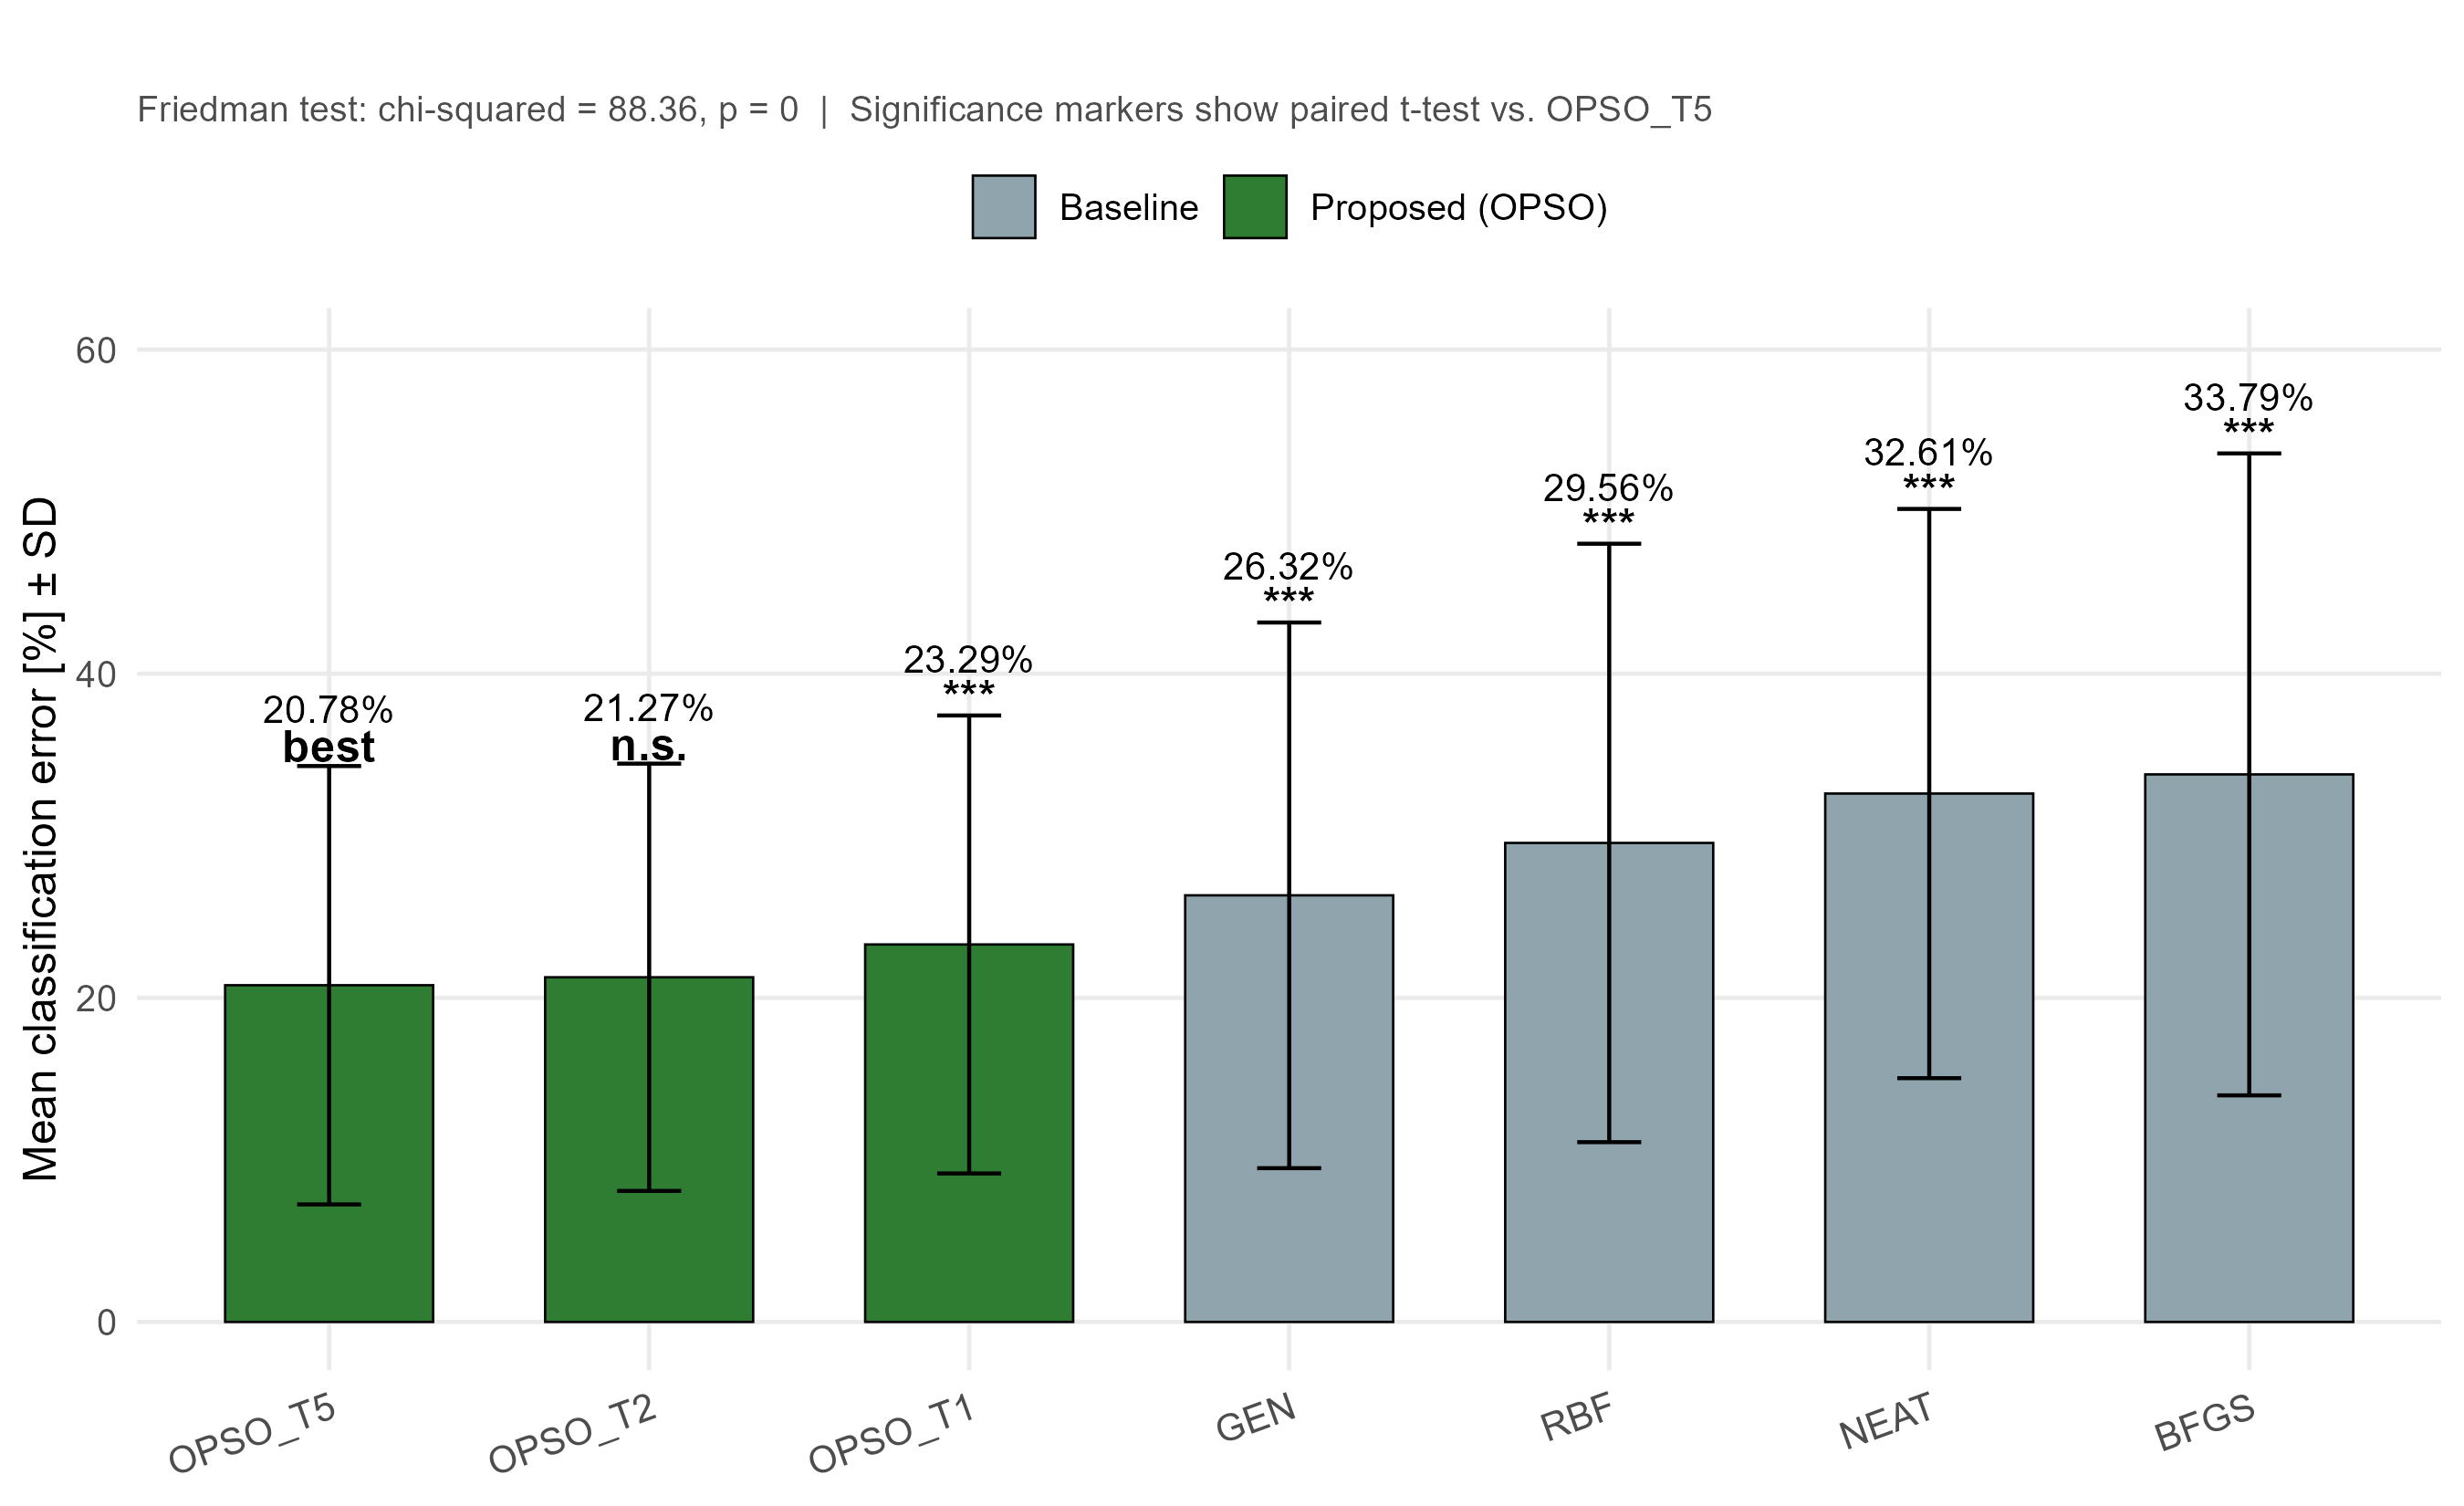
\includegraphics[scale=0.6]{tbl_basic_figure}
\par\end{centering}
\caption{Mean classification error of OPSO ($T=1,2,5$) versus baseline machine-learning
models.\label{fig:f1}}

\end{figure}

\begin{table}[H]
\caption{Statistical comparison of classification error, average ranking, and
significance tests (Wilcoxon and paired t-test) for the six machine
learning models relative to proposed method as the reference model.\label{tab:statClassification}}

\centering{}{\scriptsize{}%
\begin{tabular}{|c|c|c|c|c|c|c|c|c|c|c|}
\hline 
{\scriptsize Model} & \begin{cellvarwidth}[t]
\centering
{\scriptsize Mean}{\scriptsize\par}

{\scriptsize Error}
\end{cellvarwidth} & \begin{cellvarwidth}[t]
\centering
{\scriptsize SD}{\scriptsize\par}

{\scriptsize Error}
\end{cellvarwidth} & \begin{cellvarwidth}[t]
\centering
{\scriptsize Min}{\scriptsize\par}

{\scriptsize Error}
\end{cellvarwidth} & \begin{cellvarwidth}[t]
\centering
{\scriptsize Max}{\scriptsize\par}

{\scriptsize Error}
\end{cellvarwidth} & \begin{cellvarwidth}[t]
\centering
{\scriptsize Avg}{\scriptsize\par}

{\scriptsize Rank}
\end{cellvarwidth} & \begin{cellvarwidth}[t]
\centering
{\scriptsize Mean Diff vs}{\scriptsize\par}

{\scriptsize OPSO (T5)}
\end{cellvarwidth} & \begin{cellvarwidth}[t]
\centering
{\scriptsize Wilcoxon}{\scriptsize\par}

{\scriptsize p}
\end{cellvarwidth} & \begin{cellvarwidth}[t]
\centering
{\scriptsize Paired}{\scriptsize\par}

{\scriptsize p}
\end{cellvarwidth} & {\scriptsize Significance} & \tabularnewline
\hline 
\hline 
\begin{cellvarwidth}[t]
\centering
{\scriptsize OPSO}{\scriptsize\par}

{\scriptsize T5}
\end{cellvarwidth} & \begin{cellvarwidth}[t]
\centering
{\scriptsize Proposed}{\scriptsize\par}

{\scriptsize (OPSO)}
\end{cellvarwidth} & {\scriptsize 20.78} & {\scriptsize 13.53} & {\scriptsize 2.68} & {\scriptsize 50.67} & {\scriptsize 2.16} & {\scriptsize 0} &  &  & {\scriptsize Reference}\tabularnewline
\hline 
\begin{cellvarwidth}[t]
\centering
{\scriptsize OPSO}{\scriptsize\par}

{\scriptsize T2}
\end{cellvarwidth} & \begin{cellvarwidth}[t]
\centering
{\scriptsize Proposed}{\scriptsize\par}

{\scriptsize (OPSO)}
\end{cellvarwidth} & {\scriptsize 21.27} & {\scriptsize 13.18} & {\scriptsize 3.02} & {\scriptsize 51.97} & {\scriptsize 2.67} & {\scriptsize -0.49} & {\scriptsize 0.0351} & {\scriptsize 0.1351} & {\scriptsize n.s.}\tabularnewline
\hline 
\begin{cellvarwidth}[t]
\centering
{\scriptsize OPSO}{\scriptsize\par}

{\scriptsize T1}
\end{cellvarwidth} & \begin{cellvarwidth}[t]
\centering
{\scriptsize Proposed}{\scriptsize\par}

{\scriptsize (OPSO)}
\end{cellvarwidth} & {\scriptsize 23.29} & {\scriptsize 14.13} & {\scriptsize 3.66} & {\scriptsize 56.78} & {\scriptsize 3.58} & {\scriptsize -2.52} & {\scriptsize 0.0001} & {\scriptsize 0.0002} & {\scriptsize{*}{*}{*}}\tabularnewline
\hline 
{\scriptsize GEN} & {\scriptsize Baseline} & {\scriptsize 26.32} & {\scriptsize 16.84} & {\scriptsize 4.36} & {\scriptsize 67.81} & {\scriptsize 4.08} & {\scriptsize -5.55} & {\scriptsize 0} & {\scriptsize 0.0001} & {\scriptsize{*}{*}{*}}\tabularnewline
\hline 
{\scriptsize RBF} & {\scriptsize Baseline} & {\scriptsize 29.56} & {\scriptsize 18.46} & {\scriptsize 4.03} & {\scriptsize 71.97} & {\scriptsize 4.44} & {\scriptsize -8.78} & {\scriptsize 0.0002} & {\scriptsize 0.0002} & {\scriptsize{*}{*}{*}}\tabularnewline
\hline 
{\scriptsize NEAT} & {\scriptsize Baseline} & {\scriptsize 32.61} & {\scriptsize 17.56} & {\scriptsize 5.44} & {\scriptsize 76.19} & {\scriptsize 5.38} & {\scriptsize -11.83} & {\scriptsize 0} & {\scriptsize 0} & {\scriptsize{*}{*}{*}}\tabularnewline
\hline 
{\scriptsize BFGS} & {\scriptsize Baseline} & {\scriptsize 33.79} & {\scriptsize 19.81} & {\scriptsize 5.24} & {\scriptsize 77.55} & {\scriptsize 5.7} & {\scriptsize -13.01} & {\scriptsize 0} & {\scriptsize 0} & {\scriptsize{*}{*}{*}}\tabularnewline
\hline 
\end{tabular}}{\scriptsize\par}
\end{table}

{\scriptsize\textit{Friedman test: chi-squared = 88.36, df = 6, p-value
= 0}}{\scriptsize\par}

{\scriptsize\textit{Nemenyi critical difference (alpha = 0.05): 1.425}}{\scriptsize\par}

{\scriptsize\textit{Reference model for pairwise tests: OPSO\_T5 (auto-selected
as the best-performing OPSO variant)}}{\scriptsize\par}

{\scriptsize\textit{Significance vs. reference (paired t-test): {*}{*}{*}
p\textless 0.001, {*}{*} p\textless 0.01, {*} p\textless 0.05,
n.s. = not significant}}{\scriptsize\par}

\medskip{}

A statistical comparison of the OPSO against the other machine learning
methods is depicted in Figure \ref{fig:f1} and in Table \ref{tab:statClassification}.
Across the 40 benchmark datasets, the Friedman test revealed statistically
significant differences among the seven models under comparison$\left(\chi^{2}=88.36,\ \mbox{df}=6,\ p<0.001\right)$,
with a Nemenyi critical difference of 1.425. The OPSO variant with
$T=5$ threads achieved the lowest mean classification error (20.78\%
\textpm{} 13.53) and the best average rank (2.16), closely followed
by OPSO ($T=2$) (21.27\% \textpm{} 13.18), the difference between
the two not reaching statistical significance (paired t-test, p =
0.135). In contrast, OPSO ($T=1$) (23.29\%) and all four baseline
models, GEN (26.32\%), RBF (29.56\%), NEAT (32.61\%), and BFGS (33.79\%),
differed significantly from the best-performing variant (p \textless{}
0.001 in every case), providing strong evidence for the superiority
of the proposed OPSO algorithm, particularly under the $T=2$ and
$T=5$ configurations, over conventional approaches.

\subsection{Experiments with the propagation method\label{subsec:prop-experiments}}

Table \ref{tab:prop} reports the per-dataset classification error
obtained by the proposed OPSO algorithm under four alternative solution-propagation
strategies (NtoN, 1to1, 1toN, Nto1), evaluated across the same 40
benchmark datasets. 

\begin{table}[H]
\caption{Experiments using the proposed method and a series of propagation
techniques. The number of processing threads was set to $T=5$.\label{tab:prop}}

\centering{}%
\begin{tabular}{|c|c|c|c|c|}
\hline 
DATASET & NtoN & 1to1 & 1toN & Nto1\tabularnewline
\hline 
\hline 
APPENDICITIS & 22.80\% & 23.90\% & 23.30\% & 23.60\%\tabularnewline
\hline 
ALCOHOL & 22.13\% & 17.78\% & 20.85\% & 19.79\%\tabularnewline
\hline 
AUSTRALIAN & 24.43\% & 24.29\% & 25.19\% & 22.32\%\tabularnewline
\hline 
BALANCE & 6.94\% & 7.71\% & 8.08\% & 7.26\%\tabularnewline
\hline 
CIRCULAR & 4.34\% & 4.30\% & 4.25\% & 4.35\%\tabularnewline
\hline 
CLEVELAND & 45.69\% & 45.66\% & 47.59\% & 47.24\%\tabularnewline
\hline 
DERMATOLOGY & 9.97\% & 10.06\% & 10.40\% & 9.83\%\tabularnewline
\hline 
ECOLI & 50.67\% & 51.76\% & 50.33\% & 51.58\%\tabularnewline
\hline 
FERT & 25.50\% & 24.60\% & 25.00\% & 25.40\%\tabularnewline
\hline 
HABERMAN & 28.97\% & 29.27\% & 28.70\% & 29.53\%\tabularnewline
\hline 
HAYES ROTH & 35.00\% & 35.00\% & 37.31\% & 35.54\%\tabularnewline
\hline 
HEART & 21.11\% & 21.41\% & 20.18\% & 20.45\%\tabularnewline
\hline 
HEARTATTACK & 19.93\% & 21.53\% & 20.64\% & 21.13\%\tabularnewline
\hline 
HOUSEVOTES & 6.96\% & 6.48\% & 7.48\% & 7.61\%\tabularnewline
\hline 
IONOSPHERE & 14.86\% & 15.17\% & 15.37\% & 14.89\%\tabularnewline
\hline 
LIVERDISORDER & 31.94\% & 33.21\% & 32.47\% & 33.50\%\tabularnewline
\hline 
LYMOGRAPHY & 24.93\% & 26.07\% & 27.14\% & 26.21\%\tabularnewline
\hline 
MAMMOGRAPHIC & 17.06\% & 17.12\% & 17.19\% & 17.13\%\tabularnewline
\hline 
OPTDIGITS & 49.39\% & 49.04\% & 46.47\% & 53.38\%\tabularnewline
\hline 
PARKINSONS & 16.37\% & 15.95\% & 15.16\% & 15.90\%\tabularnewline
\hline 
PHONEME & 15.46\% & 14.91\% & 14.93\% & 14.17\%\tabularnewline
\hline 
PIMA & 27.88\% & 26.59\% & 26.92\% & 26.87\%\tabularnewline
\hline 
PIRVISION & 9.07\% & 10.52\% & 7.93\% & 9.15\%\tabularnewline
\hline 
POPFAILURES & 6.83\% & 6.80\% & 6.61\% & 7.04\%\tabularnewline
\hline 
REGIONS2 & 31.11\% & 30.73\% & 29.40\% & 30.24\%\tabularnewline
\hline 
SAHEART & 33.87\% & 33.65\% & 33.96\% & 33.15\%\tabularnewline
\hline 
SATIMAGE & 47.47\% & 52.18\% & 53.19\% & 54.45\%\tabularnewline
\hline 
SEGMENT & 17.74\% & 20.68\% & 19.07\% & 18.94\%\tabularnewline
\hline 
SONAR & 19.80\% & 22.60\% & 21.15\% & 21.90\%\tabularnewline
\hline 
SPAMBASE & 6.19\% & 6.52\% & 6.33\% & 6.09\%\tabularnewline
\hline 
SPIRAL & 41.91\% & 42.48\% & 42.22\% & 41.72\%\tabularnewline
\hline 
STATHEART & 22.22\% & 21.89\% & 23.11\% & 20.37\%\tabularnewline
\hline 
STUDENT & 5.68\% & 6.23\% & 5.90\% & 6.18\%\tabularnewline
\hline 
TRANSFUSION & 24.45\% & 24.42\% & 24.37\% & 24.29\%\tabularnewline
\hline 
WDBC & 4.95\% & 5.30\% & 6.02\% & 5.73\%\tabularnewline
\hline 
WINE & 11.82\% & 14.24\% & 13.30\% & 14.65\%\tabularnewline
\hline 
Z\_F\_S & 9.00\% & 14.40\% & 10.63\% & 13.20\%\tabularnewline
\hline 
ZO\_NF\_S & 10.08\% & 10.64\% & 8.12\% & 10.16\%\tabularnewline
\hline 
ZONF\_S & 2.68\% & 3.22\% & 2.90\% & 3.56\%\tabularnewline
\hline 
ZOO & 3.90\% & 4.50\% & 4.10\% & 5.50\%\tabularnewline
\hline 
\textbf{AVERAGE} & \textbf{20.78\%} & \textbf{21.32\%} & \textbf{21.08\%} & \textbf{21.35\%}\tabularnewline
\hline 
\end{tabular}
\end{table}

The most immediately striking behavior in this table is the remarkable
consistency of the four propagation strategies on the majority of
datasets: for cases such as BALANCE, CIRCULAR, MAMMOGRAPHIC, TRANSFUSION,
and PHONEME, the four strategies produce error values that agree to
within one or two hundredths, and in some instances within a few thousandths.
This tight clustering indicates that, for a large share of the benchmark
problems, the specific topology through which good solutions are shared
among islands has essentially no bearing on the final outcome, implying
that the search process converges to a comparable solution regardless
of how information circulates once the population size and number
of iterations are held fixed.

A markedly different behavior emerges, however, on a smaller set of
more demanding datasets. SATIMAGE shows the widest spread among all
strategies (from 0.3717 to a high of 0.5445), and comparable, if less
extreme, spreads appear for SEGMENT, WINE, Z\_F\_S, and ZO\_NF\_S.
On most of these harder cases, the full-connectivity strategy (NtoN)
tends to sit at or near the lowest error observed, consistent with
the intuition that richer, more thorough mixing of good solutions
across islands becomes increasingly valuable as the underlying optimization
landscape grows more rugged or deceptive, while restricted propagation
schemes may leave promising regions of the search space insufficiently
exploited.

At the same time, no single propagation strategy dominates uniformly
across the remaining, moderately difficult datasets: Nto1 achieves
the lowest error on AUSTRALIAN, PHONEME, and STATHEART, 1to1 is best
on HOUSEVOTES, and 1toN performs best on PARKINSONS and HEART, with
the margins separating the four strategies in each of these cases
remaining small. This idiosyncratic distribution of \textquotedbl wins\textquotedbl{}
across strategies, rather than a consistent ranking, suggests that
for datasets of intermediate difficulty the choice of propagation
topology interacts with dataset-specific characteristics in ways that
are not easily predictable from the properties of the strategy alone,
reinforcing the impression that propagation topology becomes a decisive
factor mainly at the extremes of problem difficulty rather than across
the board.

\begin{figure}[H]
\begin{centering}
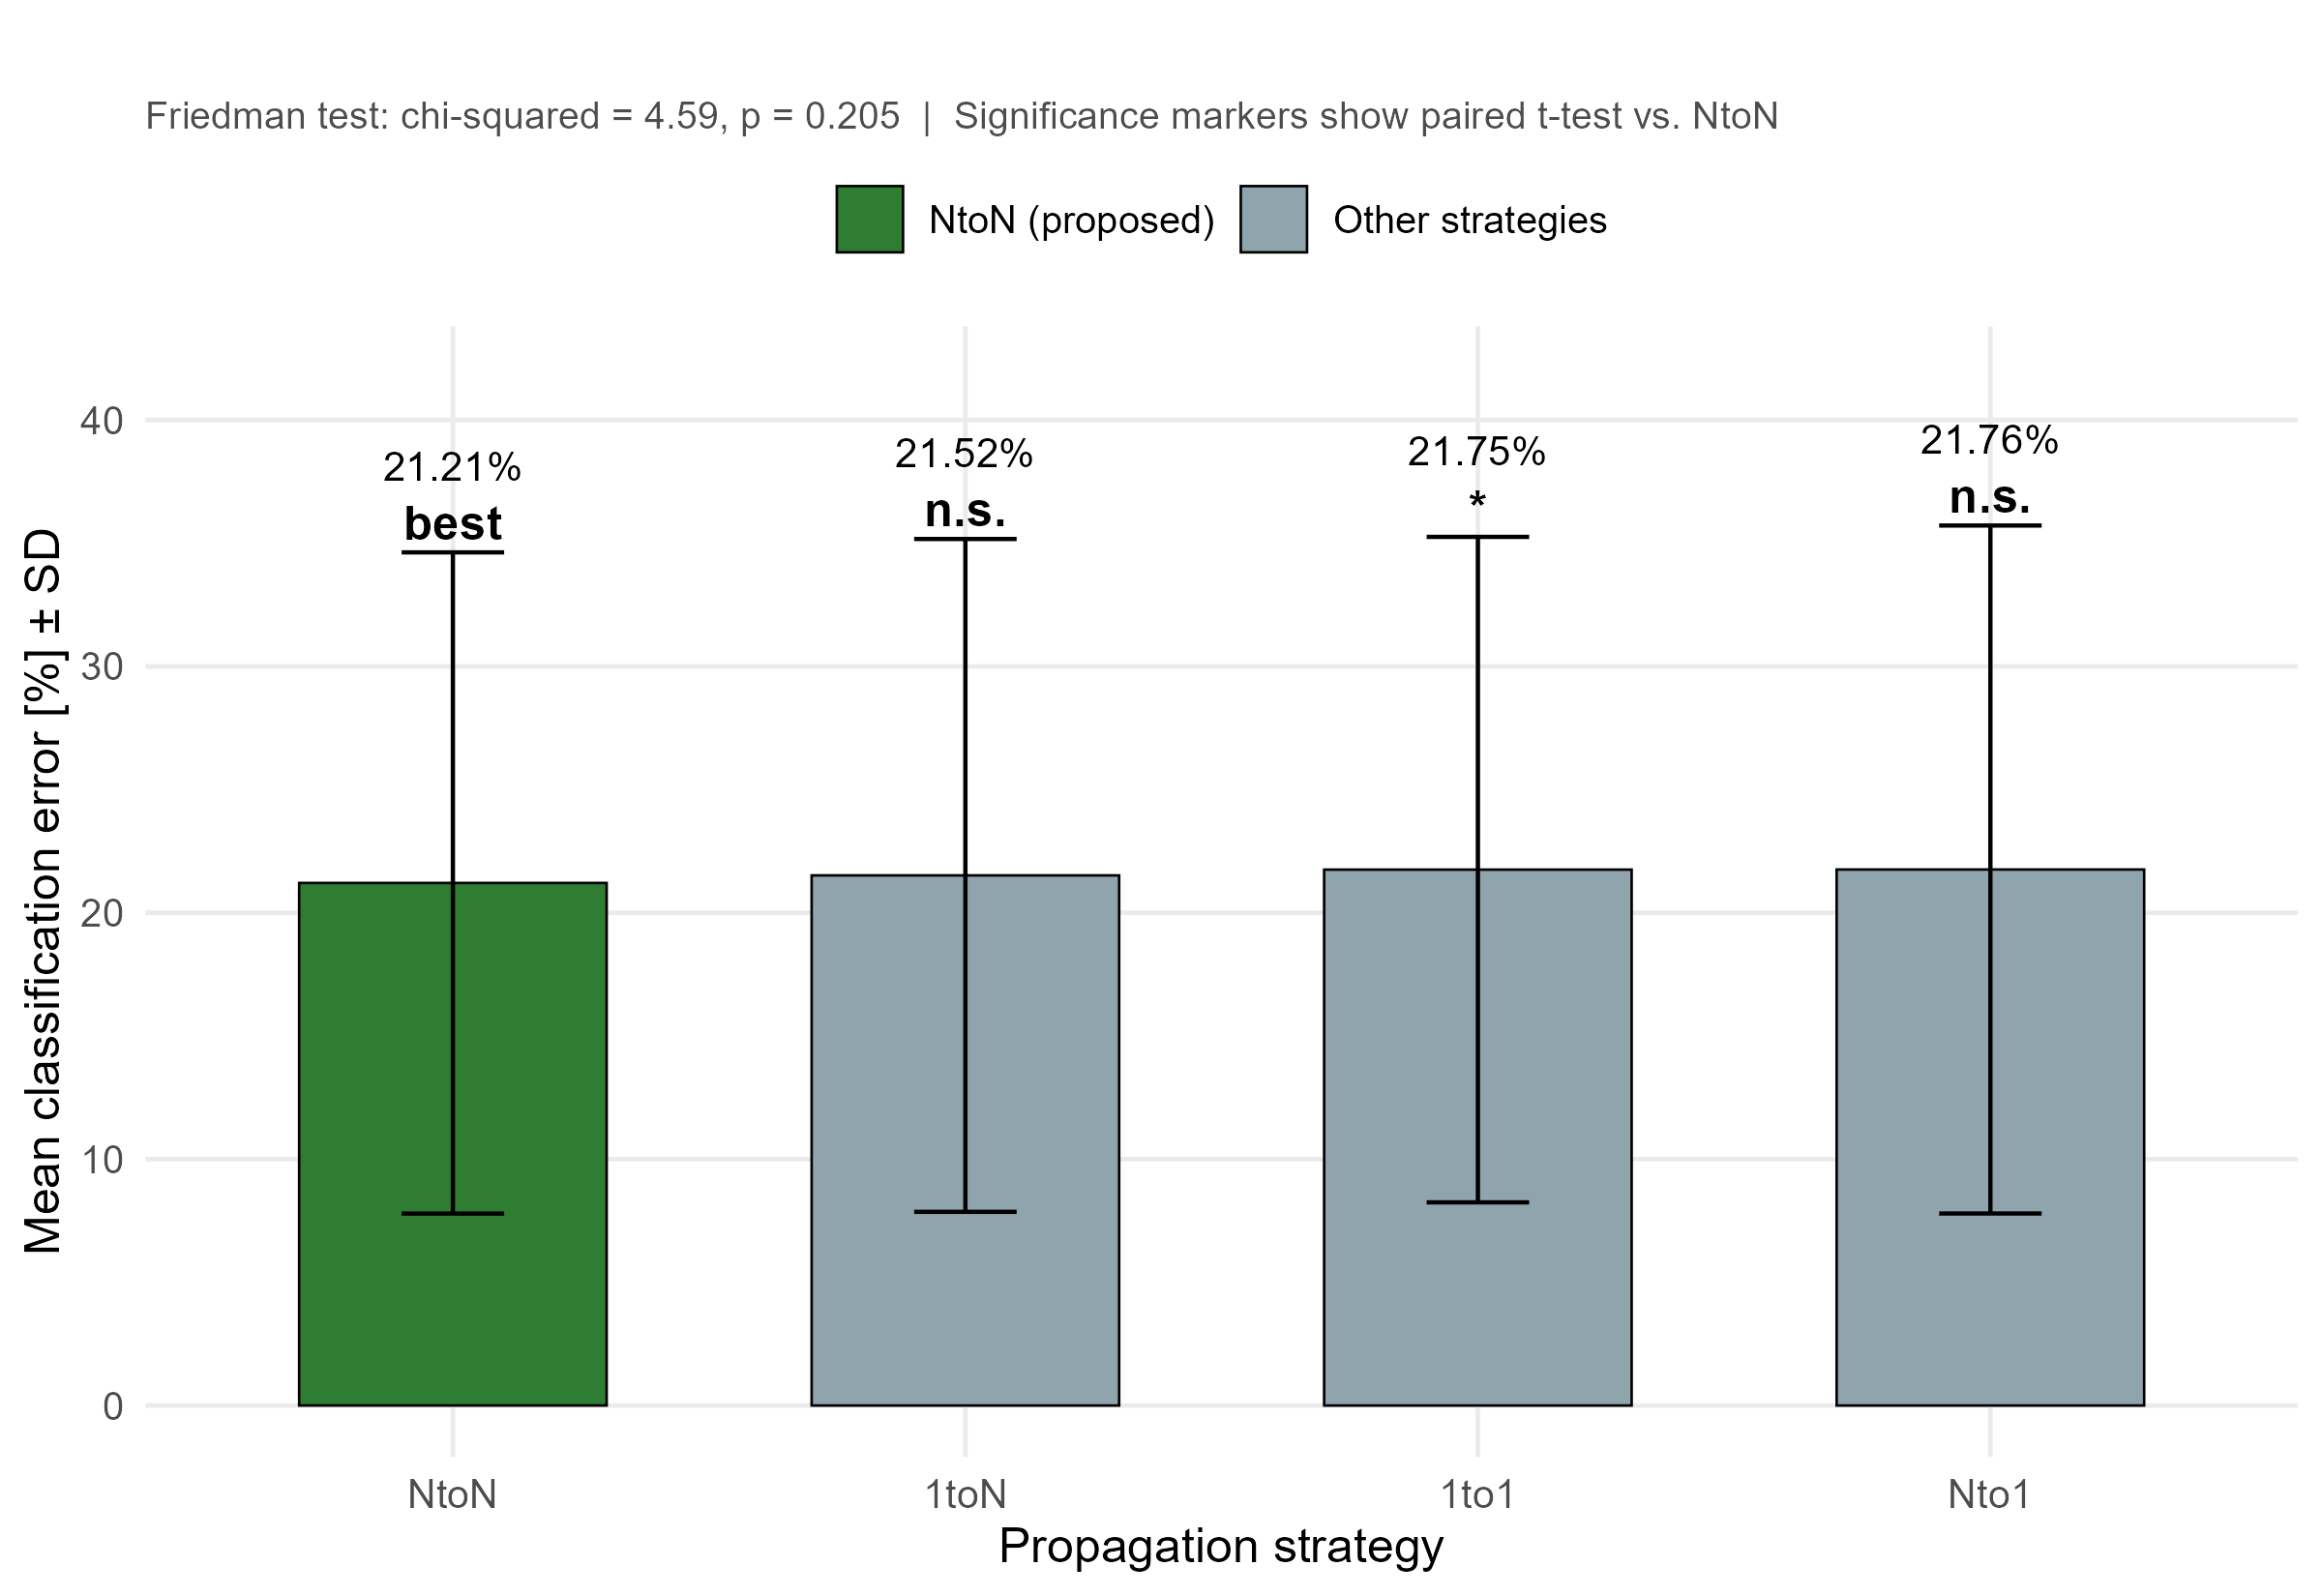
\includegraphics[scale=0.6]{tbl_prop_figure}
\par\end{centering}
\caption{Mean classification error of OPSO under four solution-propagation
strategies.\label{fig:f2}}
\end{figure}

\begin{table}[H]
\caption{Statistical comparison of the four propagation strategies relative
to NtoN.\label{tab:statProp}}

\centering{}%
\begin{tabular}{|c|c|c|c|c|c|c|c|c|c|}
\hline 
{\scriptsize Propagation} & \begin{cellvarwidth}[t]
\centering
{\scriptsize Mean}{\scriptsize\par}

{\scriptsize Error}
\end{cellvarwidth} & \begin{cellvarwidth}[t]
\centering
{\scriptsize SD}{\scriptsize\par}

{\scriptsize Error}
\end{cellvarwidth} & \begin{cellvarwidth}[t]
\centering
{\scriptsize Min}{\scriptsize\par}

{\scriptsize Error}
\end{cellvarwidth} & \begin{cellvarwidth}[t]
\centering
{\scriptsize Max}{\scriptsize\par}

{\scriptsize Error}
\end{cellvarwidth} & \begin{cellvarwidth}[t]
\centering
{\scriptsize Avg}{\scriptsize\par}

{\scriptsize Rank}
\end{cellvarwidth} & \begin{cellvarwidth}[t]
\centering
{\scriptsize Mean Diff vs}{\scriptsize\par}

{\scriptsize NtoN}
\end{cellvarwidth} & \begin{cellvarwidth}[t]
\centering
{\scriptsize Wilcoxon}{\scriptsize\par}

{\scriptsize p}
\end{cellvarwidth} & \begin{cellvarwidth}[t]
\centering
{\scriptsize Paired}{\scriptsize\par}

{\scriptsize p}
\end{cellvarwidth} & {\scriptsize Significance}\tabularnewline
\hline 
\hline 
{\scriptsize NtoN} & {\scriptsize 21.21} & {\scriptsize 13.42} & {\scriptsize 2.68} & {\scriptsize 50.67} & {\scriptsize 2.14} & {\scriptsize 0} &  &  & {\scriptsize Reference}\tabularnewline
\hline 
{\scriptsize 1toN} & {\scriptsize 21.52} & {\scriptsize 13.65} & {\scriptsize 2.9} & {\scriptsize 53.19} & {\scriptsize 2.51} & {\scriptsize -0.31} & {\scriptsize 0.1781} & {\scriptsize 0.1931} & {\scriptsize n.s.}\tabularnewline
\hline 
{\scriptsize 1to1} & {\scriptsize 21.75} & {\scriptsize 13.51} & {\scriptsize 3.22} & {\scriptsize 52.18} & {\scriptsize 2.73} & {\scriptsize -0.54} & {\scriptsize 0.0241} & {\scriptsize 0.0411} & {\scriptsize{*}}\tabularnewline
\hline 
{\scriptsize Nto1} & {\scriptsize 21.76} & {\scriptsize 13.96} & {\scriptsize 3.56} & {\scriptsize 54.45} & {\scriptsize 2.62} & {\scriptsize -0.55} & {\scriptsize 0.0874} & {\scriptsize 0.0571} & {\scriptsize n.s.}\tabularnewline
\hline 
\end{tabular}
\end{table}

{\scriptsize\textit{Friedman test: chi-squared = 4.589, df = 3, p-value
= 0.2045}}{\scriptsize\par}

{\scriptsize\textit{Nemenyi critical difference (alpha = 0.05): 0.751}}{\scriptsize\par}

{\scriptsize\textit{Reference strategy for pairwise tests: NtoN (full
propagation)}}{\scriptsize\par}

{\scriptsize\textit{Significance vs. NtoN (paired t-test): {*}{*}{*}
p\textless 0.001, {*}{*} p\textless 0.01, {*} p\textless 0.05,
n.s. = not significant}}{\scriptsize\par}

\medskip{}

A statistical comparison for the propagation strategy is depicted
in\textbf{ }Figure \ref{fig:f2} and in Table \ref{tab:statProp}.
Unlike the two preceding comparisons, the Friedman test did not detect
a statistically significant overall difference among the four propagation
strategies ($\chi^{2}$ = 4.589, df = 3, p = 0.205, n = 39, with the
summary average row excluded). The full-propagation strategy (NtoN)
attained the marginally lowest mean error (21.21\% \textpm{} 13.42)
and the best average rank (2.14), neither 1toN (21.52\%, p = 0.193)
nor Nto1 (21.76\%, p = 0.057) differed significantly from it, while
1to1 (21.75\%) showed only a nominally significant difference (p =
0.041) that does not survive correction for multiple comparisons.
Taken together, these results indicate that the topology of solution
propagation exerts a comparatively limited influence on OPSO's performance
relative to factors such as algorithmic variant or population size,
which were examined in the preceding analyses.

\subsection{Experiments with the number of particles\label{subsec:particle-experiments}}

Table \ref{tab:particles} reports the per-dataset classification
error obtained by the proposed OPSO algorithm under four different
population sizes $\left(N_{c}=200,500,1000,2000\right)$, evaluated
across the same 40 benchmark datasets. 

\begin{table}[H]
\caption{Experiments using the proposed method and a series of values for the
number of particle $N_{c}.$ The propagation method was set to $NtoN$
and the number of processing threads was set to $T=5$.\label{tab:particles}}

\centering{}%
\begin{tabular}{|c|c|c|c|c|}
\hline 
DATASET & $N_{c}=200$ & $N_{c}=500$ & $N_{c}=1000$ & $N_{c}=2000$\tabularnewline
\hline 
\hline 
APPENDICITIS & 23.70\% & 22.80\% & 21.60\% & 21.40\%\tabularnewline
\hline 
ALCOHOL & 20.42\% & 22.13\% & 18.09\% & 14.89\%\tabularnewline
\hline 
AUSTRALIAN & 23.21\% & 24.43\% & 24.78\% & 23.13\%\tabularnewline
\hline 
BALANCE & 7.19\% & 6.94\% & 7.48\% & 7.36\%\tabularnewline
\hline 
CIRCULAR & 4.35\% & 4.34\% & 4.52\% & 4.56\%\tabularnewline
\hline 
CLEVELAND & 45.41\% & 45.69\% & 45.79\% & 45.72\%\tabularnewline
\hline 
DERMATOLOGY & 13.29\% & 9.97\% & 9.92\% & 10.03\%\tabularnewline
\hline 
ECOLI & 53.70\% & 50.67\% & 49.27\% & 50.76\%\tabularnewline
\hline 
FERT & 24.30\% & 25.50\% & 27.60\% & 26.50\%\tabularnewline
\hline 
HABERMAN & 28.43\% & 28.97\% & 29.37\% & 28.97\%\tabularnewline
\hline 
HAYES ROTH & 36.00\% & 35.00\% & 36.23\% & 37.69\%\tabularnewline
\hline 
HEART & 21.14\% & 21.11\% & 19.89\% & 17.78\%\tabularnewline
\hline 
HEARTATTACK & 21.63\% & 19.93\% & 19.47\% & 19.33\%\tabularnewline
\hline 
HOUSEVOTES & 6.61\% & 6.96\% & 6.70\% & 7.30\%\tabularnewline
\hline 
IONOSPHERE & 14.71\% & 14.86\% & 15.72\% & 13.94\%\tabularnewline
\hline 
LIVERDISORDER & 34.06\% & 31.94\% & 32.47\% & 32.47\%\tabularnewline
\hline 
LYMOGRAPHY & 25.86\% & 24.93\% & 24.36\% & 25.36\%\tabularnewline
\hline 
MAMMOGRAPHIC & 16.78\% & 17.06\% & 17.29\% & 17.26\%\tabularnewline
\hline 
OPTDIGITS & 44.06\% & 49.39\% & 44.43\% & 47.46\%\tabularnewline
\hline 
PARKINSONS & 15.79\% & 16.37\% & 16.26\% & 15.05\%\tabularnewline
\hline 
PHONEME & 15.06\% & 15.46\% & 14.59\% & 15.17\%\tabularnewline
\hline 
PIMA & 29.03\% & 27.88\% & 26.62\% & 27.04\%\tabularnewline
\hline 
PIRVISION & 11.11\% & 9.07\% & 7.72\% & 8.69\%\tabularnewline
\hline 
POPFAILURES & 6.78\% & 6.83\% & 7.04\% & 6.82\%\tabularnewline
\hline 
REGIONS2 & 29.15\% & 31.11\% & 29.18\% & 27.79\%\tabularnewline
\hline 
SAHEART & 33.91\% & 33.87\% & 33.00\% & 32.67\%\tabularnewline
\hline 
SATIMAGE & 58.17\% & 47.47\% & 52.88\% & 37.17\%\tabularnewline
\hline 
SEGMENT & 19.83\% & 17.74\% & 16.46\% & 17.21\%\tabularnewline
\hline 
SONAR & 21.35\% & 19.80\% & 21.65\% & 20.15\%\tabularnewline
\hline 
SPAMBASE & 6.35\% & 6.19\% & 5.96\% & 6.33\%\tabularnewline
\hline 
SPIRAL & 42.04\% & 41.91\% & 42.41\% & 41.29\%\tabularnewline
\hline 
STATHEART & 23.96\% & 22.22\% & 21.96\% & 19.41\%\tabularnewline
\hline 
STUDENT & 6.50\% & 5.68\% & 5.45\% & 5.55\%\tabularnewline
\hline 
TRANSFUSION & 24.57\% & 24.45\% & 24.62\% & 24.16\%\tabularnewline
\hline 
WDBC & 5.61\% & 4.95\% & 5.39\% & 4.43\%\tabularnewline
\hline 
WINE & 14.12\% & 11.82\% & 10.59\% & 11.41\%\tabularnewline
\hline 
Z\_F\_S & 13.47\% & 9.00\% & 10.57\% & 8.73\%\tabularnewline
\hline 
ZO\_NF\_S & 8.68\% & 10.08\% & 6.38\% & 6.34\%\tabularnewline
\hline 
ZONF\_S & 3.16\% & 2.68\% & 2.86\% & 2.96\%\tabularnewline
\hline 
ZOO & 4.50\% & 3.90\% & 3.90\% & 4.30\%\tabularnewline
\hline 
\textbf{AVERAGE} & \textbf{21.45\%} & \textbf{20.78\%} & \textbf{20.51\%} & \textbf{19.86\%}\tabularnewline
\hline 
\end{tabular}
\end{table}

For a substantial portion of the datasets, increasing the population
size from $N_{c}=200$ to $N_{c}=2000$ produces a visible, and in
several cases fairly consistent, downward trend in error. HEART (from
0.2114 to 0.1778), STATHEART (from 0.2396 to 0.1941), HEARTATTACK
(from 0.2163 to 0.1933), and WDBC (from 0.0561 to 0.0443) all display
this steady improvement, indicating that a larger population provides
these problems with a genuinely richer sampling of the search space
that translates into more accurate final solutions rather than merely
additional computational overhead.

A second, equally prominent behavior is the near-total insensitivity
of certain datasets to population size. On MAMMOGRAPHIC, TRANSFUSION,
HABERMAN, SAHEART, CLEVELAND, BALANCE, and CIRCULAR, the error stays
within a narrow band of no more than roughly one hundredth across
all four population sizes, suggesting that for these particular problems
the search already converges to essentially the same solution with
as few as 200 individuals, and that the additional computational cost
associated with larger populations offers no discernible practical
benefit for this class of dataset.

Finally, a smaller subset of datasets displays behavior that runs
counter to the general trend, either through pronounced instability
or through outright deterioration with a larger population. SATIMAGE
stands out with the widest fluctuation observed anywhere in the table
(ranging non-monotonically from 0.5817 down to 0.3717), while FERT
(rising from 0.243 to 0.276 before partially recovering) and HAYES
ROTH (lowest at $N_{c}=500$, then rising steadily to 0.3769 at $N_{c}=2000$)
actually perform worse, on balance, with a larger population. This
behavior indicates that the relationship between population size and
solution quality is not universally monotonic, and that for certain
datasets, likely those with noisier or more deceptive fitness landscapes,
an overly large population may dilute selective pressure or slow convergence
within a fixed number of iterations, underscoring that population
size should ideally be tuned per problem rather than fixed at a single
\textquotedbl optimal\textquotedbl{} value for all datasets.

\begin{figure}[H]
\begin{centering}
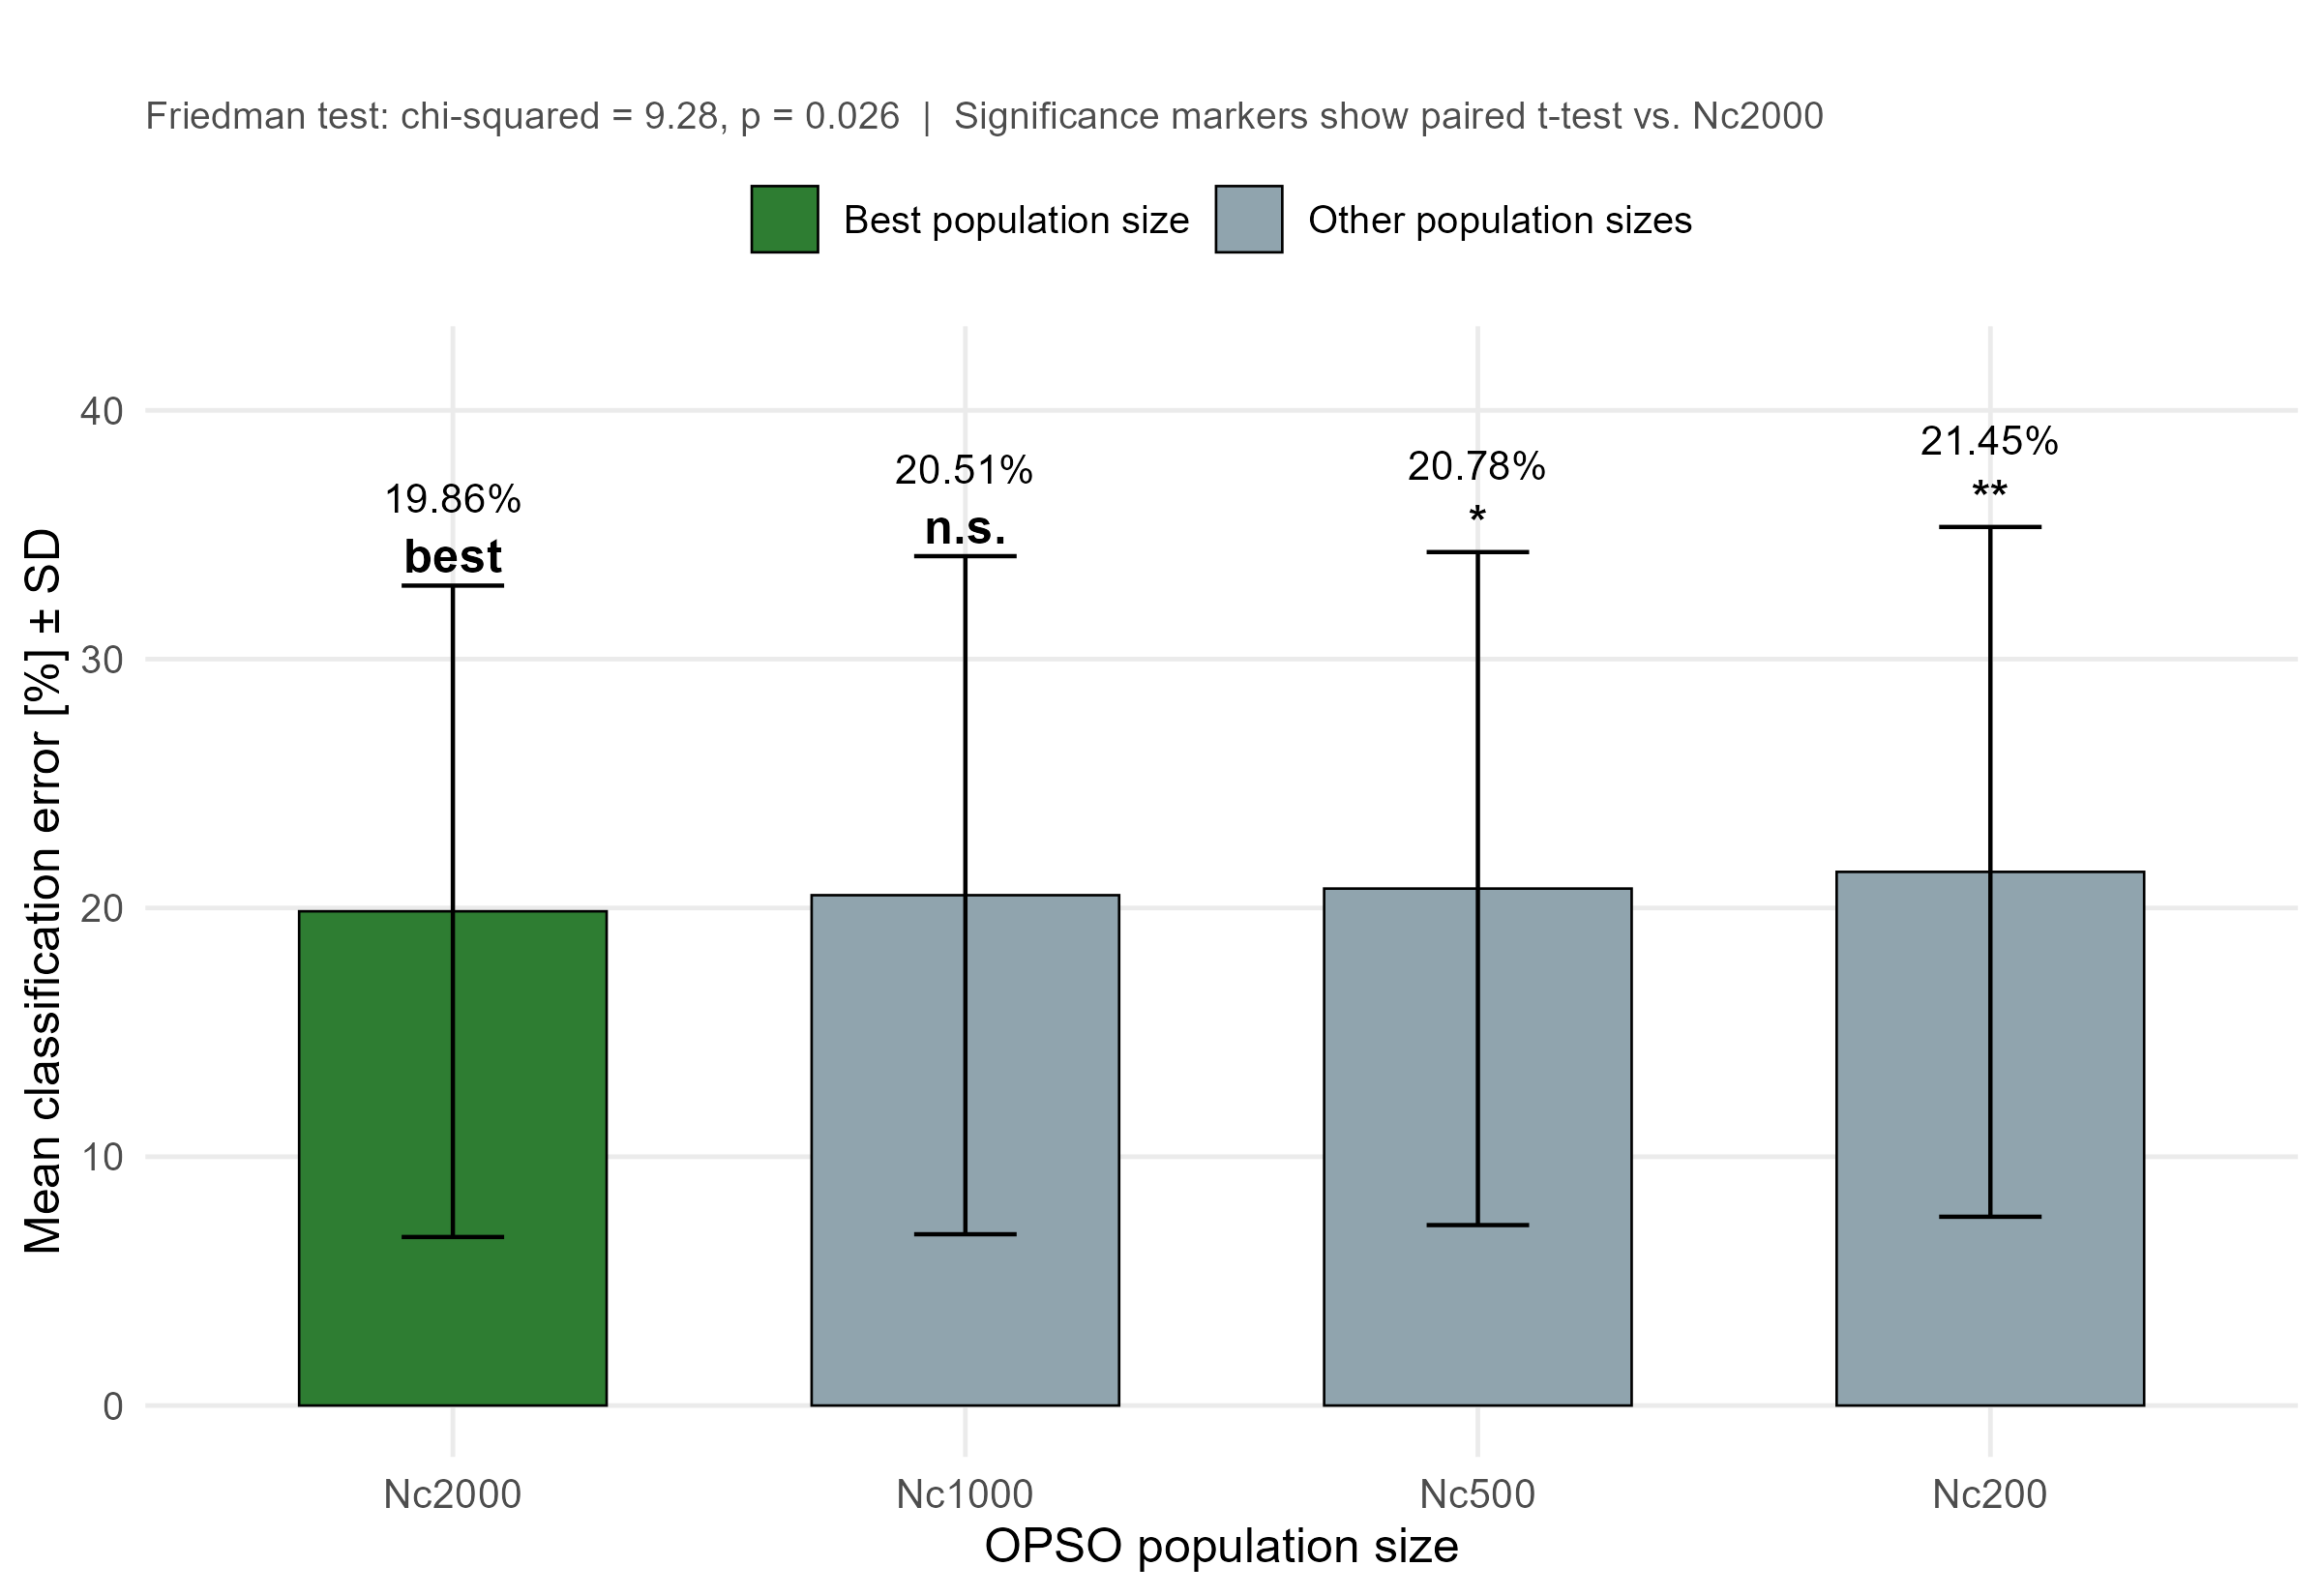
\includegraphics[scale=0.6]{tbl_part_figure}
\par\end{centering}
\caption{Mean classification error of OPSO under four population sizes.\label{fig:f3}}
\end{figure}

\begin{table}[H]
\caption{Statistical comparison of the four population sizes relative to $N_{c}$
= 2000.\label{tab:statPart}}

\centering{}%
\begin{tabular}{|c|c|c|c|c|c|c|c|c|c|}
\hline 
{\scriptsize$N_{c}$} & \begin{cellvarwidth}[t]
\centering
{\scriptsize Mean}{\scriptsize\par}

{\scriptsize Error}
\end{cellvarwidth} & \begin{cellvarwidth}[t]
\centering
{\scriptsize SD}{\scriptsize\par}

{\scriptsize Error}
\end{cellvarwidth} & \begin{cellvarwidth}[t]
\centering
{\scriptsize Min}{\scriptsize\par}

{\scriptsize Error}
\end{cellvarwidth} & \begin{cellvarwidth}[t]
\centering
{\scriptsize Max}{\scriptsize\par}

{\scriptsize Error}
\end{cellvarwidth} & \begin{cellvarwidth}[t]
\centering
{\scriptsize Avg}{\scriptsize\par}

{\scriptsize Rank}
\end{cellvarwidth} & \begin{cellvarwidth}[t]
\centering
{\scriptsize Mean Diff vs}{\scriptsize\par}

{\scriptsize$N_{c}$= 2000}
\end{cellvarwidth} & \begin{cellvarwidth}[t]
\centering
{\scriptsize Wilcoxon}{\scriptsize\par}

{\scriptsize p}
\end{cellvarwidth} & \begin{cellvarwidth}[t]
\centering
{\scriptsize Paired}{\scriptsize\par}

{\scriptsize p}
\end{cellvarwidth} & {\scriptsize Significance}\tabularnewline
\hline 
\hline 
{\scriptsize 2000} & {\scriptsize 19.86} & {\scriptsize 13.09} & {\scriptsize 2.96} & {\scriptsize 50.76} & {\scriptsize 2.08} & {\scriptsize 0} &  &  & {\scriptsize Reference}\tabularnewline
\hline 
{\scriptsize 1000} & {\scriptsize 20.51} & {\scriptsize 13.63} & {\scriptsize 2.86} & {\scriptsize 52.88} & {\scriptsize 2.48} & {\scriptsize -0.65} & {\scriptsize 0.1428} & {\scriptsize 0.1401} & {\scriptsize n.s.}\tabularnewline
\hline 
{\scriptsize 500} & {\scriptsize 20.78} & {\scriptsize 13.53} & {\scriptsize 2.68} & {\scriptsize 50.67} & {\scriptsize 2.5} & {\scriptsize -0.91} & {\scriptsize 0.0087} & {\scriptsize 0.0132} & {\scriptsize{*}}\tabularnewline
\hline 
{\scriptsize 200} & {\scriptsize 21.45} & {\scriptsize 13.86} & {\scriptsize 3.16} & {\scriptsize 58.17} & {\scriptsize 2.95} & {\scriptsize -1.59} & {\scriptsize 0.0005} & {\scriptsize 0.0089} & {\scriptsize{*}{*}}\tabularnewline
\hline 
\end{tabular}
\end{table}

{\scriptsize\textit{Friedman test: chi-squared = 9.28, df = 3, p-value
= 0.0258}}{\scriptsize\par}

{\scriptsize\textit{Nemenyi critical difference (alpha = 0.05): 0.742}}{\scriptsize\par}

{\scriptsize\textit{Reference model for pairwise tests: $N_{c}$=2000
(auto-selected as the best-performing population size)}}{\scriptsize\par}

{\scriptsize\textit{Significance vs. reference (paired t-test): {*}{*}{*}
p\textless 0.001, {*}{*} p\textless 0.01, {*} p\textless 0.05,
n.s. = not significant}}{\scriptsize\par}

\medskip{}

The statistical comparison for the obtained results is presented in
Figure \ref{fig:f3} and in Table \ref{tab:statPart}. The Friedman
test indicated an overall statistically significant effect of population
size on algorithmic performance ($\chi^{2}$ = 9.28, df = 3, p = 0.026,
n = 40), with a Nemenyi critical difference of 0.742. A population
size of $N_{c}=2000$ yielded the lowest mean error (19.86\% \textpm{}
13.09) and the best average rank (2.08), while $N_{c}=1000$ did not
differ significantly from this reference (20.51\%, p = 0.140). Smaller
populations, however, performed significantly worse: $N_{c}=500$
(20.78\%, p = 0.013) and, more markedly, $N_{c}=200$ (21.45\%, p
= 0.009). The complete, Holm-corrected pairwise comparisons (provided
as Supplementary Material) confirmed that this effect is driven primarily
by the smallest population size ($N_{c}=200$ vs. $N_{c}=1000$: paired
t-test p = 0.011 (Holm-corrected); vs. $N_{c}=2000$: p = 0.045 (Holm-corrected)),
whereas the differences among $N_{c}=500$, $N_{c}=1000$, and $N_{c}=2000$
did not remain significant after correction, suggesting diminishing
returns beyond a population size of approximately 500--1000 individuals.

\section{Conclusions\label{sec:Conclusions}}

This paper introduced OPSO, a parallel, multi-population optimization
algorithm for classification tasks, and evaluated it systematically
against four established machine-learning models across 40 benchmark
datasets drawn from the UCI and KEEL repositories. Across three thread/population
configurations, OPSO consistently and significantly outperformed all
four baseline models, with the $T=5$ configuration achieving the
lowest overall mean error and the $T=2$ configuration performing
statistically indistinguishably from it. Importantly, this advantage
was not uniform across datasets: it was most pronounced on problems
exhibiting irregular or multimodal error surfaces, precisely the class
of problems where gradient-based or single-pass heuristics are known
to struggle, while on datasets that were already comparatively easy
for the baseline models, OPSO offered little to no additional benefit.
This pattern suggests that the proposed method's principal strength
lies not in universally improving classification accuracy, but in
providing a more capable search mechanism specifically for the harder,
more deceptive regions of the problem space.

The two supplementary experiments clarified which internal design
choices of OPSO meaningfully affect its performance and which do not.
Increasing the population size produced a statistically significant
improvement, though with clearly diminishing returns beyond roughly
500--1000 particles, and with a subset of datasets showing negligible
or even mildly non-monotonic sensitivity to this parameter, indicating
that population size, while important, should be regarded as a tunable,
problem-dependent setting rather than a fixed universal choice. By
contrast, the solution-propagation strategy used to share promising
candidates among sub-populations had no statistically significant
overall effect, with the full-connectivity strategy (NtoN) offering
only a marginal, largely non-significant advantage over more restricted
topologies. Taken together, these results position OPSO as a robust
and practically competitive alternative to conventional classifier-training
approaches, whose effectiveness is driven more by the number and diversity
of its parallel search threads and the richness of its populations
than by the specific manner in which information is exchanged among
them.

The present study, while comprehensive in its comparison across baseline
models and internal configurations, leaves several directions open
for further investigation. First, the observation that OPSO's advantage
is concentrated in datasets with irregular or multimodal error landscapes
warrants a more systematic characterization of dataset difficulty,
for instance, through measures of class overlap, intrinsic dimensionality,
or landscape ruggedness, so that the conditions under which OPSO is
expected to excel can be predicted a priori rather than identified
only after the fact. Second, the non-monotonic or even adverse effect
of increasing population size observed on a small number of datasets
(e.g., FERT, HAYES ROTH) suggests that an adaptive or self-tuning
population size, adjusted dynamically during the search based on convergence
behavior, may outperform any single fixed value and merits dedicated
investigation. Third, although the propagation strategy was found
to have limited overall impact, its comparatively larger effect on
the hardest benchmark problems (e.g., SATIMAGE, SEGMENT) indicates
that hybrid or adaptive propagation schemes, which shift between restricted
and fully connected topologies depending on the observed diversity
or stagnation of the population, could yield further improvements
specifically on difficult problems, and should be explored in future
work. Finally, extending the evaluation beyond the 40 datasets considered
here to larger-scale, higher-dimensional, or streaming classification
problems, and benchmarking OPSO against a broader range of modern
evolutionary and swarm-based optimizers, would help establish the
generality of the conclusions reached in this study and clarify the
computational trade-offs involved in deploying OPSO at scale.

\vspace{6pt}


\authorcontributions{Conceptualization, K.B. and I.G.T.; methodology, K.B.; software,
K.B.; validation, V.C., G.K. and I.G.T..; formal analysis, V.C.; investigation,
I.G.T.; resources, G.K.; data curation, K.B.; writing---original
draft preparation, K.B..; writing---review and editing, I.G.T.; visualization,
V.C.; supervision, I.G.T.; project administration, I.G.T.; funding
acquisition, G.K.. All authors have read and agreed to the published
version of the manuscript.}

\funding{This research has been financed by the European Union: Next Generation
EU through the Program Greece 2.0 National Recovery and Resilience
Plan, under the call RESEARCH---CREATE---INNOVATE, project name
“iCREW: Intelligent small craft simulator for advanced crew training
using Virtual Reality techniques” (project code:TAEDK-06195).}

\institutionalreview{Not applicable.}

\informedconsent{Not applicable.}

\dataavailability{The original contributions presented in this study are included in
the article. Further inquiries can be directed to the corresponding
author.}

\conflictsofinterest{The authors declare no conflicts of interest.}

\begin{adjustwidth}{-\extralength}{0cm}{}


\reftitle{References}
\begin{thebibliography}{999}
\bibitem{Zhang2023} Zhang, A.; Lipton, Z.C.; Li, M.; Smola, A.J.
Dive into Deep Learning. \textit{arXiv} \textbf{2023}, arXiv:2106.11342v5,
\url{https://doi.org/10.48550/arXiv.2106.11342}. 

\bibitem{Kaveh2022} Kaveh, M.; Mesgari, M.S. Application of Meta-Heuristic
Algorithms for Training Neural Networks and Deep Learning Architectures:
A Comprehensive Review. \textit{Neural Process. Lett.} \textbf{2022},
\textit{54}, 1--104, \url{https://doi.org/10.1007/s11063-022-11055-6}.

\bibitem{Charilogis2024} Charilogis, V.; Kyrou, G.; Tsoulos, I.G.;
Gianni, A.M. An Innovative Hybrid Approach Producing Trial Solutions
for Global Optimization.\textit{ Appl. Sci.} \textbf{2024}, \textit{14},
10567. \url{https://doi.org/10.3390/app142210567}.

\bibitem{Dauphin2014} Dauphin, Y.N.; Pascanu, R.; Gulcehre, C.; Cho,
K.; Ganguli, S.; Bengio, Y. Identifying and attacking the saddle point
problem in high-dimensional non-convex optimization. \textit{Adv.
Neural Inf. Process. Syst.} \textbf{2014}, \textit{27}, 2933--2941.

\bibitem{Rebello2021} Rebello, C.M.; Martins, M.A.F.; Loureiro, J.M.;
Rodrigues, A.E.; Ribeiro, A.M.; Nogueira, I.B.R. From an Optimal Point
to an Optimal Region: A Novel Methodology for Optimization of Multimodal
Constrained Problems and a Novel Constrained Sliding Particle Swarm
Optimization Strategy. \textit{Mathematics} \textbf{2021}, \textit{9},
1808. \url{https://doi.org/10.3390/math9151808}

\bibitem{Metropolis1953} Metropolis, N.; Rosenbluth, A.W.; Rosenbluth,
M.N.; Teller, A.H.; Teller, E. Equation of State Calculations by Fast
Computing Machines. \textit{J. Chem. Phys}. \textbf{1953}, \textit{21},
1087--1092, \url{https://doi.org/10.1063/1.1699114}.

\bibitem{Carleo2017} Carleo, G.; Troyer, M. Solving the Quantum Many-Body
Problem with Artificial Neural Networks. \textit{Science} \textbf{2017},
\textit{355}, 602--606, \url{https://doi.org/10.1126/science.aag2302}.

\bibitem{Xia2025} Xia, X.; Zhang, Y.; Zeng, X.; Zhang, X.; Zheng,
C.; Su, Y. Artificial Intelligence in Molecular Optimization: Current
Paradigms and Future Frontiers. \textit{Int. J. Mol. Sci}. \textbf{2025},
\textit{26}, 4878. \url{https://doi.org/10.3390/ijms26104878}.

\bibitem{BuenoFerrer2025} Bueno-Ferrer, Á.; De Pablo Valenciano,
J.; De Burgos Jiménez, J. Unveiling the Potential of Metaheuristics
in Transportation: A Path Towards Efficiency, Optimization, and Intelligent
Management. \textit{Infrastructures} \textbf{2025}, \textit{10}, 4.
\url{https://doi.org/10.3390/infrastructures10010004}.

\bibitem{Andres2025}Andrès, E.; Escobar, C.; Doi, K. Machine Learning
and Artificial Intelligence in Clinical Medicine---Trends, Impact,
and Future Directions. \textit{J. Clin. Med}. \textbf{2025}, \textit{14},
8137. \url{https://doi.org/10.3390/jcm14228137}.

\bibitem{Shehata2025}Shehata, M.; Elhosseini, M. Advances in AI Technology
in Healthcare. \textit{Bioengineering} \textbf{2025}, \textit{12},
506. \url{https://doi.org/10.3390/bioengineering12050506}. 

\bibitem{Fernandez2022} Fernández, J.; G.-Tóth, B. Interval Tools
in Branch-and-Bound Methods for Global Optimization. In \textit{The
Palgrave Handbook of Operations Research}; Salhi, S., Boylan, J.,
Eds.; Palgrave Macmillan: Cham, Switzerland, \textbf{2022}; pp. 263--296,
\url{https://doi.org/10.1007/978-3-030-96935-6_8}.

\bibitem{Gillner2026}Gillner, L. Efficient acceleration strategies
for interval branch-and-bound type methods. \textit{Int. J. Approx.
Reason}. \textbf{2026}, \textit{198}, 109767, \url{https://doi.org/10.1016/j.ijar.2026.109767}.

\bibitem{Rumelhart1986}Rumelhart, D.E.; Hinton, G.E.; Williams, R.J.
Learning representations by back-propagating errors. \textit{Nature}
\textbf{1986}, \textit{323}, 533--536, \url{https://doi.org/10.1038/323533a0}.

\bibitem{Goodfellow2016}Goodfellow, I.; Bengio, Y.; Courville, A.
\textit{Deep Learning}; MIT Press: Cambridge, MA, USA, \textbf{2016}.

\bibitem{Yang2020}Yang, X.-S. \textit{Nature-Inspired Optimization
Algorithms}, 2nd ed.; Academic Press: Cambridge, MA, USA, \textbf{2020}.

\bibitem{Price1977}Price, W.L. A controlled random search procedure
for global optimisation. \textit{Comput. J.} \textbf{1977}, \textit{20},
367--370, \url{https://doi.org/10.1093/comjnl/20.4.367}.

\bibitem{Kirkpatrick1983}Kirkpatrick, S.; Gelatt, C.D., Jr.; Vecchi,
M.P. Optimization by Simulated Annealing. \textit{Science} \textbf{1983},
\textit{220}, 671--680, \url{https://doi.org/10.1126/science.220.4598.671}.

\bibitem{Kuo2022}Kuo, C.L.; Kuruoglu, E.E.; Chan, W.K.V. Neural Network
Structure Optimization by Simulated Annealing. \textit{Entropy} \textbf{2022},
\textit{24}, 348. \url{https://doi.org/10.3390/e24030348}.

\bibitem{Storn1997}Storn, R.; Price, K. Differential Evolution---A
Simple and Efficient Heuristic for Global Optimization over Continuous
Spaces. \textit{J. Glob. Optim.} \textbf{1997}, \textit{11}, 341--359,
\url{https://doi.org/10.1023/A:1008202821328}.

\bibitem{Gad2022}Gad, A.G. Particle Swarm Optimization Algorithm
and Its Applications: A Systematic Review. \textit{Arch. Comput. Methods
Eng.} \textbf{2022}, \textit{29}, 2531--2561, \url{https://doi.org/10.1007/s11831-021-09694-4}.

\bibitem{Poli2007}Poli, R.; Kennedy, J.; Blackwell, T. Particle swarm
optimization. \textit{Swarm Intell.} \textbf{2007}, \textit{1}, 33--57,
\url{https://doi.org/10.1007/s11721-007-0002-0}.

\bibitem{Dorigo2006}Dorigo, M.; Birattari, M.; Stützle, T. Ant colony
optimization. \textit{IEEE Comput. Intell. Mag. }\textbf{2006}, \textit{1},
28--39, \url{https://doi.org/10.1109/MCI.2006.329691}.

\bibitem{Holland1992}Holland, J.H. \textit{Adaptation in Natural
and Artificial Systems: An Introductory Analysis with Applications
to Biology, Control, and Artificial Intelligence}; MIT Press: Cambridge,
MA, USA, \textbf{1992}.

\bibitem{Essaid2019}Essaid, M.; Idoumghar, L.; Lepagnot, J.; Brévilliers,
M. GPU parallelization strategies for metaheuristics: a survey. \textit{Int.
J. Parallel Emergent Distrib. Syst.} \textbf{2019}, \textit{34}, 497--522,
\url{https://doi.org/10.1080/17445760.2018.1428969}.

\bibitem{Cano2016}Cano, A.; García-Martínez, C. 100 Million dimensions
large-scale global optimization using distributed GPU computing. In
\textit{Proceedings of the 2016 IEEE Congress on Evolutionary Computation
(CEC)}, \textbf{2016}; pp. 3566--3573, \url{https://doi.org/10.1109/CEC.2016.7744241}.

\bibitem{Houssein2024}Houssein, E.H.; Saeed, M.K.; Hu, G.; Ibrahim,
I.E. Metaheuristics for Solving Global and Engineering Optimization
Problems: Review, Applications, Open Issues and Challenges. \textit{Arch.
Comput. Methods Eng.} \textbf{2024}, \textit{31}, 4485--4519, \url{https://doi.org/10.1007/s11831-024-10168-6}.

\bibitem{Sun2022}Sun, Y.; Chu, S.-C.; Hu, P.; Watada, J.; Si, M.;
Pan, J.-S. Overview of Parallel Computing for Meta-Heuristic Algorithms.
\textit{J. Netw. Intell.}\textbf{ 2022}, \textit{7}, 656--684.

\bibitem{Salgotra2026}Salgotra, R.; Chaudhary, R.; Verma, P. The
Rise of Particle Swarm Optimization: A Systematic Bibliometric \&
Thematic Review (1995--2025). \textit{Arch. Comput. Methods Eng.}
\textbf{2026}, https://doi.org/10.1007/s11831-026-10532-8.

\bibitem{Rathore2017}Rathore, A.; Sharma, H. A Review on Inertia
Weight Strategies for Particle Swarm Optimization. In \textit{Proceedings
of Sixth International Conference on Soft Computing for Problem Solving};
Deep, K., Ed.; Advances in Intelligent Systems and Computing; Springer:
Singapore, \textbf{2017}; Vol. 547, pp. 88--98.

\bibitem{Charilogis2022}Charilogis, V.; Tsoulos, I.G. Toward an Ideal
Particle Swarm Optimizer for Multidimensional Functions. \textit{Information}
\textbf{2022}, \textbf{\textit{13}}, 217.

\bibitem{Demelomenezes2022}de Melo Menezes, B.A.; Kuchen, H.; Buarque
de Lima Neto, F. Parallelization of Swarm Intelligence Algorithms:
Literature Review. \textit{Int. J. Parallel Program.} \textbf{2022},
\textit{50}, 486--514, \url{https://doi.org/10.1007/s10766-022-00736-3}.

\bibitem{Charilogis2023}Charilogis, V.; Tsoulos, I.G.; Tzallas, A.
An Improved Parallel Particle Swarm Optimization. \textit{SN Comput.
Sci}. \textbf{2023},\textit{ 4}, 766. https://doi.org/10.1007/s42979-023-02227-9.

\bibitem{Nocedal2006}Nocedal, J.; Wright, S.J. \textit{Numerical
Optimization}, 2nd ed.; Springer: New York, NY, USA, \textbf{2006}.

\bibitem{Kennedy1995}Kennedy, J.; Eberhart, R. Particle swarm optimization.
In \textit{Proceedings of ICNN'95 - International Conference on Neural
Networks}, Perth, WA, Australia, \textbf{1995}; Vol. 4, pp. 1942--1948.
\url{https://doi.org/10.1109/ICNN.1995.488968}.

\bibitem{Shi1998}Shi, Y.; Eberhart, R. A modified particle swarm
optimizer. In P\textit{roceedings of the 1998 IEEE International Conference
on Evolutionary Computation Proceedings}. \textit{IEEE World Congress
on Computational Intelligence}, Anchorage, AK, USA, \textbf{1998};
pp. 69--73. \url{https://doi.org/10.1109/ICEC.1998.699146}.

\bibitem{OpenMP2024}OpenMP Architecture Review Board. \textit{OpenMP
Application Programming Interface Version 6.0}; OpenMP ARB: Beaverton,
OR, USA, \textbf{2024}. Available online: \url{https://www.openmp.org/wp-content/uploads/OpenMP-API-Specification-6-0.pdf}
(accessed on 21 July 2026).

\bibitem{Kyrou2026}Kyrou, G.; Barkas, K.G.; Charilogis, V.; Tsoulos,
I.G. Parallel Balanced Grey Wolf Optimizer: A Cooperative Parallel
Approach for Large-Scale Optimization Problems. \textit{Foundations}
\textbf{2026}, \textit{6}, 21. https://doi.org/10.3390/foundations6020021.

\bibitem{daSilveira2020}da Silveira, L.A.; Soncco-Álvarez, J.L.;
de Lima, T.A.; Ayala-Rincón, M. Behavior of Bioinspired Algorithms
in Parallel Island Models. In \textit{Proceedings of the 2020 IEEE
Congress on Evolutionary Computation (CEC)}, Glasgow, UK, \textbf{2020};
pp. 1--8. \url{https://doi.org/10.1109/CEC48606.2020.9185732}.

\bibitem{Abadlia2017}Abadlia, H.; Smairi, N.; Ghedira, K. Particle
swarm optimization based on island models. In \textit{Proceedings
of the Genetic and Evolutionary Computation Conference Companion};
Association for Computing Machinery: New York, NY, USA,\textbf{ 2017};
pp. 101--102. \url{https://doi.org/10.1145/3067695.3076068}.

\bibitem{Tsoulos2021}Tsoulos, I.G.; Tzallas, A.; Karvounis, E. Improving
the PSO method for global optimization problems. \textit{Evolving
Systems} \textbf{2021}, \textit{12}, 875--883. \url{https://doi.org/10.1007/s12530-020-09330-9}.

\bibitem{Petalas2007}Petalas, Y.G.; Parsopoulos, K.E.; Vrahatis,
M.N. Memetic particle swarm optimization. \textit{Ann. Oper. Res.}
\textbf{2007}, \textit{156}, 99--127. \url{https://doi.org/10.1007/s10479-007-0224-y.}

\bibitem[(1989)]{uci} M. Kelly, R. Longjohn, K. Nottingham, The UCI
Machine Learning Repository, \url{https://archive.ics.uci.edu}.

\bibitem{Keel}J. Alcalá-Fdez, A. Fernandez, J. Luengo, J. Derrac,
S. García, L. Sánchez, F. Herrera. KEEL Data-Mining Software Tool:
Data Set Repository, Integration of Algorithms and Experimental Analysis
Framework. Journal of Multiple-Valued Logic and Soft Computing 17,
pp. 255-287, 2011.

\bibitem{appendicitis}Weiss, Sholom M. and Kulikowski, Casimir A.,
Computer Systems That Learn: Classification and Prediction Methods
from Statistics, Neural Nets, Machine Learning, and Expert Systems,
Morgan Kaufmann Publishers Inc, 1991.

\bibitem[Tzimourta(2018)]{alcohol}Tzimourta, K.D.; Tsoulos, I.; Bilero,
I.T.; Tzallas, A.T.; Tsipouras, M.G.; Giannakeas, N. Direct Assessment
of Alcohol Consumption in Mental State Using Brain Computer Interfaces
and Grammatical Evolution. Inventions 2018, 3, 51.

\bibitem{australian}J.R. Quinlan, Simplifying Decision Trees. International
Journal of Man-Machine Studies \textbf{27}, pp. 221-234, 1987. 

\bibitem{balance}T. Shultz, D. Mareschal, W. Schmidt, Modeling Cognitive
Development on Balance Scale Phenomena, Machine Learning \textbf{16},
pp. 59-88, 1994.

\bibitem{cleveland1}Z.H. Zhou,Y. Jiang, NeC4.5: neural ensemble based
C4.5,\textquotedbl{} in IEEE Transactions on Knowledge and Data Engineering
\textbf{16}, pp. 770-773, 2004.

\bibitem{cleveland2}R. Setiono , W.K. Leow, FERNN: An Algorithm for
Fast Extraction of Rules from Neural Networks, Applied Intelligence
\textbf{12}, pp. 15-25, 2000.

\bibitem{dermatology}G. Demiroz, H.A. Govenir, N. Ilter, Learning
Differential Diagnosis of Eryhemato-Squamous Diseases using Voting
Feature Intervals, Artificial Intelligence in Medicine. \textbf{13},
pp. 147--165, 1998.

\bibitem[(1996)]{ecoli}P. Horton, K.Nakai, A Probabilistic Classification
System for Predicting the Cellular Localization Sites of Proteins,
In: Proceedings of International Conference on Intelligent Systems
for Molecular Biology \textbf{4}, pp. 109-15, 1996.

\bibitem{hayesroth}B. Hayes-Roth, B., F. Hayes-Roth. Concept learning
and the recognition and classification of exemplars. Journal of Verbal
Learning and Verbal Behavior \textbf{16}, pp. 321-338, 1977.

\bibitem{heart}I. Kononenko, E. Šimec, M. Robnik-Šikonja, Overcoming
the Myopia of Inductive Learning Algorithms with RELIEFF, Applied
Intelligence \textbf{7}, pp. 39--55, 1997

\bibitem{housevotes}R.M. French, N. Chater, Using noise to compute
error surfaces in connectionist networks: a novel means of reducing
catastrophic forgetting, Neural Comput. \textbf{14}, pp. 1755-1769,
2002.

\bibitem{ion1}J.G. Dy , C.E. Brodley, Feature Selection for Unsupervised
Learning, The Journal of Machine Learning Research \textbf{5}, pp
845--889, 2004.

\bibitem{ion2}S. J. Perantonis, V. Virvilis, Input Feature Extraction
for Multilayered Perceptrons Using Supervised Principal Component
Analysis, Neural Processing Letters \textbf{10}, pp 243--252, 1999.

\bibitem{liver} J. Garcke, M. Griebel, Classification with sparse
grids using simplicial basis functions, Intell. Data Anal. \textbf{6},
pp. 483-502, 2002.

\bibitem[(2002)]{lymography}G. Cestnik, I. Konenenko, I. Bratko,
Assistant-86: A Knowledge-Elicitation Tool for Sophisticated Users.
In: Bratko, I. and Lavrac, N., Eds., Progress in Machine Learning,
Sigma Press, Wilmslow, pp. 31-45, 1987. 

\bibitem{mammographic}M. Elter, R. Schulz-Wendtland, T. Wittenberg,
The prediction of breast cancer biopsy outcomes using two CAD approaches
that both emphasize an intelligible decision process, Med Phys. \textbf{34},
pp. 4164-72, 2007.

\bibitem{parkinsons}Little MA, McSharry PE, Hunter EJ, Spielman J,
Ramig LO. Suitability of dysphonia measurements for telemonitoring
of Parkinson's disease. IEEE Trans Biomed Eng. 2009;56(4):1015. doi:10.1109/TBME.2008.2005954

\bibitem{pima}J.W. Smith, J.E. Everhart, W.C. Dickson, W.C. Knowler,
R.S. Johannes, Using the ADAP learning algorithm to forecast the onset
of diabetes mellitus, In: Proceedings of the Symposium on Computer
Applications and Medical Care IEEE Computer Society Press, pp.261-265,
1988.

\bibitem[(2023)]{pirvision}Emad-Ud-Din, M., \& Wang, Y. (2023). Promoting
occupancy detection accuracy using on-device lifelong learning. IEEE
Sensors Journal, 23(9), 9595-9606.

\bibitem{popfailures}D.D. Lucas, R. Klein, J. Tannahill, D. Ivanova,
S. Brandon, D. Domyancic, Y. Zhang, Failure analysis of parameter-induced
simulation crashes in climate models, Geoscientific Model Development
\textbf{6}, pp. 1157-1171, 2013.

\bibitem{regions}Giannakeas, N., Tsipouras, M.G., Tzallas, A.T.,
Kyriakidi, K., Tsianou, Z.E., Manousou, P., Hall, A., Karvounis, E.C.,
Tsianos, V., Tsianos, E. A clustering based method for collagen proportional
area extraction in liver biopsy images (2015) Proceedings of the Annual
International Conference of the IEEE Engineering in Medicine and Biology
Society, EMBS, 2015-November, art. no. 7319047, pp. 3097-3100. 

\bibitem{saheart}T. Hastie, R. Tibshirani, Non-parametric logistic
and proportional odds regression, JRSS-C (Applied Statistics) \textbf{36},
pp. 260--276, 1987.

\bibitem{segment}M. Dash, H. Liu, P. Scheuermann, K. L. Tan, Fast
hierarchical clustering and its validation, Data \& Knowledge Engineering
\textbf{44}, pp 109--138, 2003.

\bibitem[(1988)]{sonar}Gorman, R.P.; Sejnowski, T.J. Analysis of
Hidden Units in a Layered Network Trained to Classify Sonar Targets.
Neural Netw. 1988, 1, 75--89.

\bibitem[(2000)]{spambase}Cranor, Lorrie F., LaMacchia, Brian A.
Spam!, Communications of the ACM, 41(8):74-83, 1998.

\bibitem[(2007)]{student}P. Cortez, A. M. Gonçalves Silva, Using
data mining to predict secondary school student performance, In Proceedings
of 5th FUture BUsiness TEChnology Conference (FUBUTEC 2008) (pp. 5--12).
EUROSIS-ETI, 2008.

\bibitem[(2007)]{transfusion}I-Cheng Yeh, King-Jang Yang, Tao-Ming
Ting, Knowledge discovery on RFM model using Bernoulli sequence, Expert
Systems with Applications \textbf{36}, pp. 5866-5871, 2009.

\bibitem{wdbc}W.H. Wolberg, O.L. Mangasarian, Multisurface method
of pattern separation for medical diagnosis applied to breast cytology,
Proc Natl Acad Sci U S A. \textbf{87}, pp. 9193--9196, 1990.

\bibitem{wine1}M. Raymer, T.E. Doom, L.A. Kuhn, W.F. Punch, Knowledge
discovery in medical and biological datasets using a hybrid Bayes
classifier/evolutionary algorithm. IEEE transactions on systems, man,
and cybernetics. Part B, Cybernetics : a publication of the IEEE Systems,
Man, and Cybernetics Society, \textbf{33} , pp. 802-813, 2003.

\bibitem{wine2}P. Zhong, M. Fukushima, Regularized nonsmooth Newton
method for multi-class support vector machines, Optimization Methods
and Software \textbf{22}, pp. 225-236, 2007.

\bibitem{eeg}R.G. Andrzejak, K. Lehnertz, F. Mormann, C. Rieke, P.
David, and C. E. Elger, Indications of nonlinear deterministic and
finite-dimensional structures in time series of brain electrical activity:
Dependence on recording region and brain state, Phys. Rev. E \textbf{64},
pp. 1-8, 2001.

\bibitem{zoo}M. Koivisto, K. Sood, Exact Bayesian Structure Discovery
in Bayesian Networks, The Journal of Machine Learning Research\textbf{
5}, pp. 549--573, 2004.

\bibitem[(2022)]{optimus}Tsoulos, I. G., Charilogis, V., Kyrou, G.,
Stavrou, V. N., \& Tzallas, A. (2025). OPTIMUS: A Multidimensional
Global Optimization Package. Journal of Open Source Software, 10(108),
7584.

\bibitem[(2025)]{bfgs}Yuan, Y. X. (1991). A modified BFGS algorithm
for unconstrained optimization. IMA Journal of Numerical Analysis,
11(3), 325-332.

\bibitem{nn1}C. Bishop, Neural Networks for Pattern Recognition,
Oxford University Press, 1995.

\bibitem{nn2}G. Cybenko, Approximation by superpositions of a sigmoidal
function, Mathematics of Control Signals and Systems \textbf{2}, pp.
303-314, 1989.

\bibitem[(2025)]{neat}K. O. Stanley, R. Miikkulainen, Evolving Neural
Networks through Augmenting Topologies, Evolutionary Computation \textbf{10},
pp. 99-127, 2002.

\bibitem[(1991)]{rbf1}J. Park and I. W. Sandberg, Universal Approximation
Using Radial-Basis-Function Networks, Neural Computation \textbf{3},
pp. 246-257, 1991.

\bibitem{rbf2}G.A. Montazer, D. Giveki, M. Karami, H. Rastegar, Radial
basis function neural networks: A review. Comput. Rev. J \textbf{1},
pp. 52-74, 2018.

\bibitem{geneticnn1}Reynolds, J., Rezgui, Y., Kwan, A., \& Piriou,
S. (2018). A zone-level, building energy optimisation combining an
artificial neural network, a genetic algorithm, and model predictive
control. Energy, 151, 729-739.

\end{thebibliography}
%%%%%%%%%%%%%%%%%%%%%%%%%%%%%%%%%%%%%%%%%%
%% for journal Sci
%\reviewreports{\\
%Reviewer 1 comments and authors' response\\
%Reviewer 2 comments and authors' response\\
%Reviewer 3 comments and authors' response
%}
%%%%%%%%%%%%%%%%%%%%%%%%%%%%%%%%%%%%%%%%%%

\PublishersNote{}

\end{adjustwidth}{}
\end{document}
